\documentclass[oneside]{book}
\usepackage[a4paper, top=3cm, bottom=3cm]{geometry}
\usepackage[latin1]{inputenc}
\usepackage{setspace}
\usepackage{fancyhdr}
\usepackage{tocloft}
\usepackage{graphicx}
\usepackage{listings}
\usepackage{sectsty}

%\usepackage{helvet}
%\renewcommand{\familydefault}{\sfdefault}
\fontsize{12pt}{20pt}
\selectfont

\addtolength{\parskip}{\baselineskip}
\begin{document}
\setlength{\parindent}{0in}


\pagestyle{empty}
%\pagenumbering{}
% Set book title
\title{\textbf{Hazelcast}}
% Include Author name and Copyright holder name
\author{Peter Veentjer}

% 1st page for the Title
%-------------------------------------------------------------------------------
\maketitle


% 2nd page, thanks message
%-------------------------------------------------------------------------------
\thispagestyle{empty}
Hazelcast
Peter Veentjer.
\newpage

% General definitions for all Chapters
%-------------------------------------------------------------------------------

% Define Page style for all chapters
\pagestyle{fancy}
% Delete the current section for header and footer
\fancyhf{}
% Set custom header
\lhead[]{\thepage}
\rhead[\thepage]{}

% Set arabic (1,2,3...) page numbering
\pagenumbering{arabic}

% Set double spacing for the text
%\doublespacing

% If the chapter ends in an odd page, you may want to skip having the page
%  number in the empty page
% \thispagestyle{empty}


\chapter*{Pragmatic Bookshelf}
Many of the designations used by manufacturers and sellers to distinguish their products are claimed as trademarks. 
Where those designations appear in this book, and The Pragmatic Programmers, LLC was aware of a trademark claim, the 
designations have been printed in initial capital letters or in all capitals. The Pragmatic Starter Kit, The Pragmatic 
Programmer, Pragmatic Programming, Pragmatic Bookshelf, PragProg and the linking g device are trade- marks of The 
Pragmatic Programmers, LLC.

Every precaution was taken in the preparation of this book. However, the publisher assumes no responsibility for 
errors or omissions, or for damages that may result from the use of information (including program listings) contained herein.
Our Pragmatic courses, workshops, and other products can help you and your team create better software and have more fun. 

For more information, as well as the latest Pragmatic titles, please visit us at http://pragprog.com.
The team that produced this book includes:
\begin{enumerate}
\item people
\end{enumerate}

\chapter*{Acknowledgments}

Lorem ipsum dolor sit amet, consectetur adipiscing elit. Morbi libero sem,
interdum eget varius vel, faucibus placerat purus. Sed vulputate diam sit amet
risus dapibus dignissim. Praesent lobortis eleifend augue. Cum sociis natoque
penatibus et magnis dis parturient montes, nascetur ridiculus mus. Morbi libero
turpis, viverra ac vulputate a, faucibus vel quam. Quisque interdum congue
lacus, in tempus nisl tincidunt at. Curabitur sed eros eu enim vehicula
fermentum quis nec justo. Vestibulum rutrum laoreet est, eget condimentum justo
feugiat at. Cras ac sem ac magna ornare tempor non nec nisl. Maecenas feugiat
fringilla nisl, vitae ullamcorper ante posuere a. Sed mollis lacinia interdum.
Vivamus vel urna metus. Nulla eget tellus sem. Praesent volutpat suscipit nulla,
nec dictum arcu iaculis id. Duis pharetra vestibulum sapien, quis pulvinar odio
pharetra id. Cras at erat velit, vel tincidunt elit. Curabitur vehicula leo eu
odio vulputate ac consequat nulla ultricies. Maecenas venenatis condimentum
urna ut ultrices. Aliquam blandit fermentum eros, ac lacinia sem scelerisque
at. Nullam vitae nisi at erat posuere cursus a non velit.

\chapter*{Preface}
Writing concurrent system has been a long passion of mine and it is a very logical step to go from concurrency control within a single JVM to concurrency control over multiple JVM's. There is a big overlap in functionality; a lot of the knowledge that is applicable to concurrency control in a single JVM also applies to concurrency over multiple JVM's; but there also is a whole new dimension of problems that make distributed systems even more interesting to deal with. 
\subsection*{What is Hazelcast}
When you write applications for the JVM for your profession, it is likely that you are going to write server-side applications. Although Java has support for writing desktop applications, the server-side is really where Java shines.

Today, especially with the introduction of cloud computing, it becomes more and more important that server-side systems are:
\begin{enumerate}
\item Scalable: just add and remove machines to match required capacity 
\item Highly available: if one or more machines in a system fail, the system should continue as if nothing happened.
\item High performing: the performance per machine should be good enough to make it cost efficient.
\end{enumerate}

Hazelcast is an Open Source clustering and highly scalable data distribution platform for the JVM. It is:
\begin{enumerate}
\item Dynamically scalable: This is done by making certain Hazelcast data-structures - like Hazelcast Map - partitioned so that partitions can be spread evenly among the members. When members join or leave the cluster, Hazelcast will automatically move partitions from one member to another.
\item Highly available: It does not lose data after a JVM crash. This is done by automatically replicating partition data on other cluster members. In case of a member going down, the system will automatically failover by restoring the backup. Another important design feature of Hazelcast is that there is no master member that can form a single point of failure; each member has equal responsibilities.
\item Lightning-fast: Each Hazelcast member can do thousands of operations per second.
\end{enumerate}
Hazelcast will not automatically spawn additional JVM's to become members in the cluster when the load exceeds a certain upper threshold because this is very environment specific so it will not fit you in a once size fits all solution. For the same reason it will not shutdown JVM's when the load exceeds a certain lower threshold.

One of the things I like most about Hazelcast is that it isn't very intrusive; as a developer/architect you are in control how much Hazelcast you get in your system. You are not forced to mutilate objects so they can be distributed, forced to use specific (application) servers or complex api's or the need to install software; just add the Hazelcast jar to your classpath and you are done.

This freedom combined with very well thought out API's, in a lot of cases you can just use interfaces like java.util.concurrent.Executor, java.util.concurrent.BlockingQueue or java.util.Map, makes Hazelcast really a joy to work with. So it helps you with implementing highly available, scalable and high-performing systems, written in little time and based on very simple and elegant code.

\subsection*{Who should read this book}
This books aims at developers/architects that build applications on top of the JVM and want to get a better understanding of how to write distributed applications using Hazelcast. It doesn't matter if you are using Java or any other the other JVM based languages like Scala, Groovy, Clojure. It is even possible to call Hazelcast from .NET or C++ using the new Hazelcast 3 Portable and client functionality.

If you are a developer that has no prior experience with Hazelcast, then you will learn the basics to get up and running. If you already have some experience, it might be that you learn some new tricks since the book contains a lot of information that is not (yet) part of the Hazelcast manual.
 
\subsection*{What is in this book}
This book shows you how to make use of Hazelcast by going through most important features. It also includes the newest Hazelcast 3 improvements. Some of these improvements are minor changes, but can have a huge impact on a system. Others are very big like the SPI which makes it possible to write your own distributed data-structures if you are not happy with the ones provided by Hazelcast.

In 'Chapter 1: Learning the Basics', you will learn how to download and set up Hazelcast and to create a basic project. You will also learn about some of the general Hazelcast concepts.

In 'Chapter 2: Distributed Primitives', you will learn how to use basic concurrency primitives like ILock, IAtomicLong, IdGenerator, ISemaphore and ICountDownLatch and about their advanced settings.

In 'Chapter 3: Distributed Collections', you will learn how to make use of distributed collections like the IQueue, IList and ISet.

In 'Chapter 4: Distributed Map', you will learn about the IMap functionality. Since its functionality is very extensive, there is a whole topic about dealing with its configuration options like high availability, scalability etc. You will also learn how to use Hazelcast as a cache and persist its values.

In 'Chapter 5: Distributed Executor', you will learn about executing tasks using the distributed Executor. By using  the executor you turn Hazelcast into a computing grid. 

In 'Chapter 6: Distributed Topic', you will learn about creating a publish/subscribe solution using the Distributed Topic functionality.

In 'Chapter 7: Hazelcast clients', you will learn about connecting to a Hazelcast cluster as a client. This topic not only deals with creating a client but also with more complex features like loadbalancing and failover.

In 'Chapter 8: Serialization', you will learn more about the different serialization technologies that are supported by Hazelcast. Not only Java Serializable and Externalizable will be explained, but also the native Hazelcast serialization techniques like DataSerializable and the new Portable functionality.

In 'Chapter 9: Transactions', you will learn about Hazelcast's transaction support to prevent transactional data-structures from being left in inconsistent state.

After that in 'Chapter 10: Network Configuration', you will learn about Hazelcast's network configuration. You will learn about different member discovery mechanism like multicast, Amazon EC2 and security. 

Next in 'Chapter 11: SPI', you will learn about using the Hazelcast SPI to make first class distributed services yourself. This functionality perhaps is the most important new feature of Hazelcast 3.0.

Finally in 'Chapter 12: Performance', you will learn more about performance tuning.  Out of the box a lot data-structures like the map have all kinds of default settings that are perhaps good for certain situations, like high availability, but could be impacting your performance. 

\subsection*{What you need}
In Order to use Hazelcast you'll need a computer that is able to run Java 5+. If you don't have Java installed on your machine, you will probably want to install Java 7: 
http://www.oracle.com/technetwork/java/javase/downloads/index.html. 

To build the code examples for this book, make sure that Maven 3 is installed. Which can be downloaded from the following website: http://maven.apache.org.

Apart from Java and Maven, you can use your favorite IDE, e.g. Eclipse or IntelliJ, to view and edit the code and to run the examples. 

\subsection*{Online resources}
There is a website for this book that contains a link to an interactive discussion forum and you can submit your errata to the book here as well. Also the Java source code and the configuration files can be found here. 

The Hazelcast website and various other useful sites can be found here:
\begin{enumerate}
\item Hazelcast Website: http://hazelcast.com/
\item Hazelcast Documentation: http://hazelcast.com/docs.jsp
\item Hazelcast Usergroup: http://groups.google.com/group/hazelcast
\item Hazelcast on Github: https://github.com/hazelcast/hazelcast/
\end{enumerate}
Building distributed systems on Hazelcast is really joy to do and I hope I can make you as enthusiastic about it as I am. So lets get started with building distributed applications you can be proud of.

\newpage

% Last pages for ToC
%-------------------------------------------------------------------------------
% Include dots between chapter name and page number
\renewcommand{\cftchapdotsep}{\cftdotsep}

\tableofcontents

\chapter{Learning the basics}
In this chapter we'll learn very basics to getting started; so downloading Hazelcast, configuring Hazelcast in a Maven project. And we'll also deal with the different configuration mechanisms of Hazelcast and configuration tricks like wildcard configuration.

\section{Installing Hazelcast}
Hazelcast relies on Java 5, but the examples rely on Java 7. So if you want to compile the examples, make sure Java 7 is installed. If not installed, it can be downloaded from the Oracle site: http://java.com/en/download/index.jsp.

Hazelcast can be downloaded from http://www.hazelcast.com/downloads.jsp and you can choose between 2 versions:
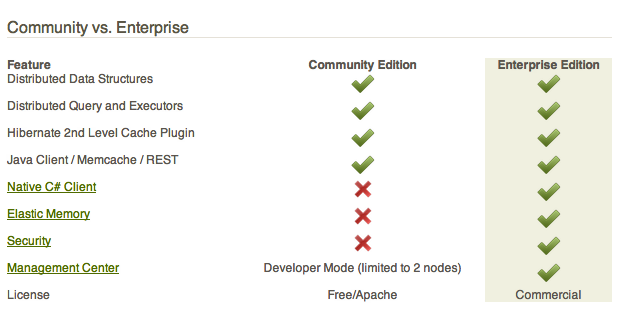
\includegraphics[scale=0.60]{hazelcast-editions.png}
For the purpose of this book we'll use the community edition. If your project relies on Maven, there is no need to install Hazelcast at all, see [link to Hazelcast and Maven]. Otherwise make sure that the Hazelcast jar is added to the classpath. Apart from this jar, there is no need to install Hazelcast.  The lack of an installation process for Hazelcast is something I really like because it saves quite a lot of time, time that can be used to solve real problems instead of environmental ones.

\section{Hazelcast and Maven}
Hazelcast is very easy to include in your Maven 3 project without needing to go through a complex installation process. Hazelcast can be found in the standard Maven repositories, so you do not need to add additional repositories to the pom. To include Hazelcast in your project, just add the following to your pom:
\begin{lstlisting}[language=xml]
<dependencies>	
    <dependency>
      <groupId>com.hazelcast</groupId>
      <artifactId>hazelcast</artifactId>
      <version>3.0</version>
   </dependency>
</dependencies>
\end{lstlisting}
That is it. Make sure that you check the Hazelcast website to make use of the most recent version. After this dependency is added, Maven will automatically downloaded the dependencies needed.

\section{Configuring Hazelcast}
Hazelcast can be configured in different ways:
\begin{enumerate}
\item programmatic configuration
\item XML configuration 
\item Spring configuration
\end{enumerate}
The programmatic configuration is the most essential one, the other mechanisms are build on top of it. In this book we'll use the xml configuration file since that is the shortest. When you are running a Maven project; just add a resources directory under src/main/ and add a file 'hazelcast.xml'. The following shows an empty configuration:
\begin{lstlisting}[language=xml]
<hazelcast xsi:schemaLocation="http://www.hazelcast.com/schema/config
                               http://www.hazelcast.com/schema/config/hazelcast-config-3.0.xsd"
           xmlns="http://www.hazelcast.com/schema/config"
           xmlns:xsi="http://www.w3.org/2001/XMLSchema-instance">
</hazelcast>
\end{lstlisting}
This example also imports an XML schema (XSD) for validation and if you are using an IDE, you probably get code completion. To reduce the size of the examples in the book, only the elements inside the <hazelcast> tags are provided. In the sources for the book you can find the full xml configuration. Another thing you might run into is the strange formatting of the java code; this is also done to reduce the size. 

In most of our examples we will rely on multicast for member discovery so that the members will join the cluster:
\begin{lstlisting}[language=xml]
<network>
   <join><multicast enabled="true"/></join>
</network>
\end{lstlisting}
See [chapter Cluster Configuration: Multicast] if multicast doesn't work or you want to know more about it. If you are using the programmatic configuration, then multicast is enabled by default.

In this book, the following approach is used to create a new Hazelcast instance:
\begin{lstlisting}[language=java]
public class Main {
    public static void main(String[] args){
        HazelcastInstance hzInstance = Hazelcast.newHazelcastInstance();
        ...
    }
}
\end{lstlisting}
The mechanism uses the following alternatives to resolve the configuration:
\begin{enumerate}
\item first checks if the 'hazelcast.config' system property is set; if it is, then the value is used as path. This is useful if you want to choose on startup of the application which hazelcast configuration file should be used. The config option can be set by adding the following to the java command: '-Dhazelcast.config=<path to the hazelcast.xml>'. The value can be a normal file path, but can also be a classpath reference if it is prefixed with 'classpath:'. 
\item else it checks if there is a 'hazelcast.xml' in the working directory.
\item after that it check if there is a 'hazelcast.xml' on the classpath. 
\item finally loads the default hazelcast configuration 'hazelcast-default.xml' that is part of the Hazelcast jar
\end{enumerate}
Also be careful to check the Hazelcast output when you are relying on an hazelcast.xml file. If it contains errors, Hazelcast will not abort the startup but will default to the 'hazelcast-default.xml'. When this happens, the system could behave completely different than you would expect.

Another option to load a HazelcastInstance, is to make use of programmatic configuration, e.g: 
\begin{lstlisting}[language=java]
public class Main {
    public static void main(String[] args){
       ExecutorConfig executorConfig = new ExecutorConfig().setPoolSize(10);
       Config config = new Config().addExecutorConfig(executorConfig);	  
       HazelcastInstance hzInstance = Hazelcast.newHazelcastInstance(config);
       ...
    }
}
\end{lstlisting}
The Hazelcast Config object has a fluent interface; meaning that the Config instance is returned when a config method on this instance is called. This makes chaining method calls very easy. The programmatic configuration is not only very useful for testing, but it also a solution for the static nature of the XML configuration. The content of the programmatic configuration can easily be created on the fly, e.g. based on database content. You could even decide to move the 'static' configuration to the hazelcast.xml, load this and then modify the dynamic parts, e.g. the network configuration.

In Hazelcast releases prior to 3.0, there was functionality for a static default HazelcastInstance, so you could say: 'Queue q = Hazelcast.getQueue("foo")'. This functionality has been removed because it lead to confusion when explicit created HazelcastInstances are combined with calls to the implicit default HazelcastInstance. So you probably want to keep a handle to the Hazelcast instance somewhere for future usage.

\section{Wildcard configuration}
The Hazelcast xml configuration can contain configuration elements for all kinds of distributed data-structures: sets, executors, maps etc. For example:
\begin{lstlisting}[language=xml]
<map name="testmap">
    <time-to-live-seconds>10</time-to-live-seconds>
</map>
\end{lstlisting}
But what if we want to create multiple map instances using the same configuration? Do we need to configure them individually? This is impossible to do if you have a dynamic number of distributed data-structures and you don't know up front how many need to be created. The solution to this problem is wildcard configuration, which is available for all data-structures. This makes it possible to use the same configuration for multiple instances. For example, we could configure the previous 'testmap' example with a 10 'time-to-live-seconds' using a wildcard configuration like this:
\begin{lstlisting}[language=xml]
<map name="testmap*">
   <time-to-live-seconds>10</time-to-live-seconds>
</map>
\end{lstlisting}
Using a single asterisk (*) character any place in the name, the same configuration can be shared by different  data-structures. The wildcard configuration can be used like this:
\begin{lstlisting}[language=java]
     Map map1 = hzInstance.getMap("testmap1");
     Map map2 = hzInstance.getMap("testmap2");
\end{lstlisting}
The maps 'testmap1' and 'testmap2' both match 'testmap*' so they will use the same configuration.

Something thing you need to watch out for are multiple configurations that match. Hazelcast will not throw an error or log a warning. Also selecting the right configuration doesn't depend on the order of definition in the configuration file and also isn't based on the best fitting match. So really make sure that your wildcard configurations are very specific. One of the ways to do it is to include the package name:
\begin{lstlisting}[language=xml]
<map name="com.foo.testmap*">
    <time-to-live-seconds>10</time-to-live-seconds>
</map>
\end{lstlisting}
A map can be loaded calling 'Map map1 = hzInstance.getMap("com.foo.testmap1")'. 

\section{Multiple Hazelcast instances}
In most cases you will have a single Hazelcast Instance per JVM. But Multiple Hazelcast Instances can run in a single JVM. This is not only useful for testing, but also for more complex setups e.g. application servers running multiple independent applications that rely on Hazelcast. Multiple Hazelcast instances can be started like this:
\begin{lstlisting}[language=java]
public class MultipleMembers {
    public static void main(String[] args){
        HazelcastInstance hzInstance1 = Hazelcast.newHazelcastInstance();
        HazelcastInstance hzInstance2 = Hazelcast.newHazelcastInstance();}}
\end{lstlisting}
When you start this multiple members, you see something like this in the output:
\begin{lstlisting}
Members [2] {
    Member [192.168.1.100]:5701 this
    Member [192.168.1.100]:5702
}
...
Members [2] {
    Member [192.168.1.100]:5701
    Member [192.168.1.100]:5702 this
}
\end{lstlisting}
As you can see there is a 2 member cluster created.

\section{Properties}
In the Hazelcast xml file properties can be included like this:
\begin{lstlisting}[language=xml]
<properties>
    <property name="property-name">property-value</property>
</properties>
\end{lstlisting}
 Apart from properties in the hazelcast.xml, they can also be passed on the commandline 'java -Dproperty-name=property-value'. One thing to watch out for; you can't override properties from the hazelcast.xml/programmatic-configuration from the command line because the latter has a lower priority. For a full listing of available properties see the 'Advanced configuration' chapter of the Hazelcast reference manual.

\section{Import}
[todo:this functionality is not yet implemented in Hazelcast 3]

\section{Variables}
[todo:this functionality is not yet implemented in Hazelcast 3]

\section{Logging}
Hazelcast supports various logging mechanisms; 'jdk', 'log4', 'sl4j' or 'none' if you don't want to have any logging. The default is 'jdk': the logging that is part of the JRE, so no additional dependencies are needed. Logging can be set by adding a property in the hazelcast.xml:
\begin{lstlisting}[language=xml]
<properties>
    <property name="hazelcast.logging.type">log4j</property>
</properties>
\end{lstlisting}
Or if you are using the programmatic configuration:
\begin{lstlisting}[language=java]
Config cfg = new Config() ;
cfg.setProperty("hazelcast.logging.type", "log4j");
\end{lstlisting}
But it can also be configured from the command line using: 'java -Dhazelcast.logging.type=log4j'. If you are going to make use of 'log4j' or 'slf4j', make sure that the correct dependencies are included. See the examples sources for more information.

If you are not satisfied with the provided logging implementations, you can always implement your own logging implementation by implementing the 'com.hazelcast.logging.LogListener'. See the Hazelcast reference manual for more information.

\section{Downloading example sources}
If you want to play around with the example sources of this book, check the following link:[todo: link to source]. 

\section{What is next?}
Hazelcast supports a lot of functionality, so we cover only the most used functionality. Some things like named HazelcastInstances have been left out. [todo: more content?]
\chapter{Distributed Primitives}
If you have programmed in Java you have probably worked with concurrency primitives like the synchronized statement (the intrinsic lock) or perhaps even the concurrency library that was introduced in Java 5 under java.util.concurrent like the Executor, Lock and AtomicReference.

This concurrency functionality is useful if you want to write a Java application that use multiple threads, but the focus is to provide is synchronization in a single JVM and not distributed over multiple JVM's. Luckily Hazelcast provides support for various distributed synchronization primitives like the Lock, IAtomicLong etc. And apart from making synchronization between different JVM's possible, they also support high availably; so if one machine fails, the primitive remains usable for other JVM's.

\section{IAtomicLong}
The IAtomicLong, formally known as the AtomicNumber, is the distributed version of the java.util.concurrent.atomic.AtomicLong, so if you have used that before, working with the IAtomicLong should feel very similar. The IAtomicLong exposes most of the operations the AtomicLong provides like get, set, getAndSet, compareAndSet and incrementAndGet, but there is of course a big difference in performance since remote calls are involved.

I'll demonstrate the IAtomicLong by creating an instance and incrementing it one million times:
\begin{lstlisting}[language=java]
public class Member {
   public static void main(String[] args) {
      HazelcastInstance hz = Hazelcast.newHazelcastInstance();
      IAtomicLong counter = hz.getAtomicLong("counter");
      for (int k = 0; k < 1000 * 1000; k++) {
         if (k % 500000 == 0) 
            System.out.println("At: "+k);
         counter.incrementAndGet();
      }
      System.out.printf("Count is %s\n", counter.get());
   }
}
\end{lstlisting}
If you start this Member, you will see this:
\begin{lstlisting}
At: 0
At: 500000
Count is 1000000
\end{lstlisting}
If you run multiple instances of this member, then the total count should be equal to one million times the number of members you have started.

If the IAtomicLong becomes a contention point in your system, there are a few ways of dealing with it, depending on your requirements. One of the options it to create a stripe (essentially an array) of IAtomicLong instances to reduce pressure. Another options is to keep changes local and only publish them to the IAtomicLong once and a while. There are a few downsides here; you could loose information if a member goes down and is that the newest value is not always immediately visible to the outside world. If you want to generate unique id's, you can have a look at the IdGenerator.

Hazelcast only provides support for the long, but you can always simulate other types:
\begin{enumerate}
\item boolean: 0 for true and 1 for false.
\item double: a 64 bit double can be encoded into 64 bits, which can be stored in a long since is also 64 bits.
\end{enumerate}
There is no support for an atomic reference, but if you need it you can build it on top of the IMap. The name of the reference could be the key and the value could be the reference value. The IMap implements the ConcurrentMap interface, so you can lift on atomic operations like replace(K key, V oldValue, V newValue). 

\section{IdGenerator}
In previous section the IAtomicLong was introduced and one of the things it can be used for is to generated unique id's within a cluster. Although it will work, it probably isn't the most scalable solution since all member will content on incrementing the value. If you are only interested in unique id's you can have a look at the com.hazelcast.core.IdGenerator.

The way the IdGenerator works is that each member claims a segment of 1 million id's to generate. This is done behind the scenes by using an IAtomicLong and claiming a segment is done by incrementing that IAtomicLong by a million. After claiming the segment, the IdGenerator can increment a local counter. Once all id's in the segment are used, it needs to claim a new segment. The consequence of this approach is that only 1 in a million times network traffic is needed; so 999.999 out of 1.000.000 the id generation can be done in memory and therefor is extremely fast. Another consequence is that this approach scales a lot better than an IAtomicLong because there is a lot less contention: 1 out of 1.000.000 instead of 1 out of 1.

So lets see the IdGenerator in action:
\begin{lstlisting}[language=java]
public class IdGeneratorMember {
   public static void main(String[] args) throws Exception{
      HazelcastInstance hz = Hazelcast.newHazelcastInstance();
      IdGenerator idGenerator = hz.getIdGenerator("id");
      for (int k = 0; k < 1000; k++){
         Thread.sleep(1000);
         System.out.printf("Id : %s\n", idGenerator.newId());
      }
   }
}
\end{lstlisting}
If you start this multiple times, you will see in the console that there will not be any duplicate id's.

Of course there are some issues you need to be aware of:
\begin{enumerate}
\item id's generated by different members will be out of order
\item if a member goes down without fully using its segment, there might be gaps.
\end{enumerate}
For id generation, in most cases, this isn't not relevant. There are alternative solutions for creating cluster wide unique id's. One of them is the java.util.UUID, although it will take up more space than a long, it doesn't rely on access to a Hazelcast cluster.

Another important issue you need to know is that if the cluster restarts, then the IdGenerator is reset and starts from 0 because the IdGenerator doesn't write to storage, e.g a database. If you need this, you can create your own IdGenerator based on the same implementation mechanism the IdGenerator uses, but you persist the updates to the IAtomicLong.

\section{ILock}
A lock is a synchronization primitive that makes it possible that only a single thread is able to access to a critical section of code; if multiple threads at the same moment would access that critical section concurrently, you would get race problems. 

Hazelcast provides a distributed lock implementation and makes it possible to create a critical section within a cluster of JVM's; so only a single thread from one of the JVM's in the cluster is allowed to acquire that lock. Other threads that want to acquire the lock, no matter if they are on the same JVM's or not, will not be able to acquire it and depending on the locking method they called, they either block or fail. The com.hazelcast.core.ILock extends the java.util.concurrent.locks.Lock interface, so using the lock is quite simple.

The following example shows how a lock can be used to solve a race problem:
\begin{lstlisting}[language=java]
public class RaceFreeMember {
   public static void main(String[] args) throws Exception {
      HazelcastInstance hz = Hazelcast.newHazelcastInstance();
      IAtomicLong number1 = hz.getAtomicLong("number1");
      IAtomicLong number2 = hz.getAtomicLong("number2");
      ILock lock = hi.getLock("lock");
      System.out.println("Started");
      for (int k = 0; k < 10000; k++) {
         if (k % 100 == 0) 
            System.out.println("at: " + k);
         lock.lock();
         try {
            if (k % 2 == 0) {
               long n1 = number1.get();
               Thread.sleep(10);
               long n2 = number2.get();
               if (n1 - n2 != 0) 
                  System.out.println("Datarace detected!");
               } else {
                    number1.incrementAndGet();
                    number2.incrementAndGet();
               }
         } finally {lock.unlock();}
      }
      System.out.println("Finished");
   }
}
\end{lstlisting}
When this code is executed; you will not see "Datarace detected!". This is because the lock provides a critical section around writing and reading of the numbers. In the example code you will also find the version with a data race.

A few things worth knowing about the Hazelcast lock and locking in general:
\begin{enumerate}
\item It is reentrant, so you can acquire it multiple times in a single thread without causing a deadlock, of course you need to release it as many times as you have acquired it, to make it available to other threads.
\item Just like with the other Lock implementations, it should always be acquired outside of a try/finally block. Else it can happen that the lock acquire failed, but an unlock is still executed. 
\item Keep locks as short as possible. If locks are kept too long, it can lead to performance problems or worse: deadlock.
\item With locks it is easy to run into deadlocks if you don't know what you are doing; so make sure that you do. Having code you don't control running inside your locks is asking for problems. Make sure you understand exactly the scope of the lock. 
\item To reduce the chance of a deadlock, the tryLock methods can be used that control the waiting period. The lock.lock() method will not block indefinitely, but will timeout with a OperationTimeoutException after 300 seconds.  
\item Locks are automatically released when a member has acquired a lock and this member goes down. This prevents threads that are waiting for a lock to wait indefinitely and needed for failover to work in a distributed system. The downside however is that if a member goes down that acquired the lock and started making changes, that other members could start to see partial changes. In these cases either the system could do some self repair or else a transaction potentially can solve the problem.
\item a lock must always be released by the same lock that acquired it, otherwise look at the ISemaphore.
\item locks are fair, so locks will be granted in the order they are requested.
\item there are no configuration options available for the lock
\item you can ask the lock if it is locked using the ILock.isLocked method.
\item a lock can be forced to unlock using the ILock.unlock method. This should be used with extreme care since it could stop a critical section from being locked. 
\end{enumerate}

[todo: lock doesn't work on name, but can be any object.. important to realize that it isn't the monitor lock of that particular 'name' you are acquiring]

\section{ICondition}
One of the new features of Hazelcast 3 is support for the ICondition which extends the java.util.concurrent.locks.Condition. Each lock can have mulitple conditions (e.g. queue full, queue empty) There is 1 difference, with the normal Java version you can create condition and depends on its reference to identify which condition you are waiting for. With Hazelcast this isn't possible since different members can't share a object reference. That is why an id is needed to identify the condition.

\begin{lstlisting}[language=java]
public class WaitingMember {
   public static void main(String[] args) throws InterruptedException {
      HazelcastInstance hz = Hazelcast.newHazelcastInstance();
      IAtomicLong counter = hz.getAtomicLong("counter");
      ILock lock = hz.getLock("lock");
      System.out.println("Starting wait");
      ICondition condition = lock.newCondition("condition");
      lock.lock();
      try {
         while (counter.get() != 1) {
            condition.await();
         }
      } finally {
         lock.unlock();
      }
      System.out.println("Wait finished");
   }
}
\end{lstlisting}

\begin{lstlisting}[language=java]
public class NotifyMember {
   public static void main(String[] args) throws InterruptedException {
      HazelcastInstance hz = Hazelcast.newHazelcastInstance();
      IAtomicLong counter = hz.getAtomicLong("counter");
      ILock lock = hz.getLock("lock");
      ICondition condition = lock.newCondition("condition");
      lock.lock();
      try {
         counter.set(1);
         condition.signalAll();
      } finally {
         lock.unlock();
      }
   }
}
\end{lstlisting}

spurious wakeups. 
signal vs signallAll

\section{ISemaphore}
The semaphore is a classic synchronization aid that can be used to control the number of threads doing a certain activity concurrently, e.g. using a resource. Conceptually each semaphore has a number of permits, where each permit represents a single thread allowed to execute that activity concurrently. As soon as a thread want to start with the activity, it takes a permit (or waits until one becomes available) and once finished with the activity, the permit is returned.

If you initialize the semaphore with a single permit, it looks a lot like a lock. One of the big difference is that the Semaphore has no concept of ownership. So with a lock the thread that acquired the lock must release it, but with a semaphore any thread can release an acquired permit. Another difference is that an exclusive lock only has 1 permit and a semaphore can have more than 1.

Hazelcast provides a distributed version of the java.util.concurrent.Semaphore named the com.hazelcast.core.ISemaphore. When a permit is acquired on the ISemaphore the following can happen:
\begin{enumerate}
\item a permit is available. The number of permits in the semaphore is decreased by one and the calling thread can continue. 
\item no permit is available. The calling thread will block until a permit comes available, a timeout happens, the thread is interrupted or when the semaphore is destroyed an InstanceDestroyedException will be thrown.
\end{enumerate}
I'll explain the semaphore with an example. To simulate a shared resource we have an IAtomicLong initialized with the value 0. This resource is going to used 1000 times, When a thread starts to use that resource it increments it and once completed it decrements it.
\begin{lstlisting}[language=java]
public class SemaphoreMember {
   public static void main(String[] args)throws Exception{
      HazelcastInstance hz = Hazelcast.newHazelcastInstance();
      ISemaphore semaphore = hz.getSemaphore("semaphore");
      IAtomicLong resource = hz.getAtomicLong("resource");
      for(int k=0;k<1000;k++){
         System.out.println("At iteration: "+k +
            ", Active Threads: " + resource.get());
         semaphore.acquire();
         try{
            resource.incrementAndGet();
            Thread.sleep(1000);
            resource.decrementAndGet();
         }finally{semaphore.release();}
      }
      System.out.println("Finished");
   }
}
\end{lstlisting}
We want to limit the concurrent access to the resource by allowing for at most 3 thread. This can be done by configuring the initial-permits for the semaphore in the Hazelcast config file:
\begin{lstlisting}[language=xml]
<semaphore name="semaphore">
   <initial-permits>3</initial-permits>
</semaphore>
\end{lstlisting}
When you start the SemaphoreMember 5 times you will see output like this:
\begin{lstlisting}
At iteration: 0, Active Threads: 1
At iteration: 1, Active Threads: 2
At iteration: 2, Active Threads: 3
At iteration: 3, Active Threads: 3
At iteration: 4, Active Threads: 3
\end{lstlisting}
As you can see the maximum number of concurrent threads using that resource always is equal or smaller than 3. As an experiment you can remove the semaphore acquire/release statements and see for yourself that there is no longer control on the number of concurrent usages of the resources.

A few things worth knowing about the ISemaphore:
\begin{enumerate}
\item fairness: the Semaphore acquire methods are fair and this is not configurable. So under contention, the longest waiting thread for a permit will acquire it before all other threads. This is done to prevent starvation, at the expense of reduced throughput.
\item attach permits: one of the features added to the ISemaphore to make it more reliable in a distributed environment where failover is important, is the addition of attached permits. Normally when a permit is acquired, and the member that acquired the permit goes down, the permit is not released. The consequence is that the permit is lost and the maximum number of concurrent threads for a specific activity is reduced. It can even lead to a deadlock situation when the number of available permits reaches 0. With the attached permits, the permit is attached to a member, and when it goes down, the permit is automatically released (similar as with the Hazelcast Lock).
\item the acquire() method doesn't timeout, unlike the Hazelcast Lock.lock() method. To prevent running into a deadlock, using one of timed acquire methods is a good solution.
\end{enumerate}

[TODO: Semaphore factory.]

\section{ICountDownLatch}
The java.util.concurrent.CountDownLatch was introduced in Java 1.5 and is a synchronization aid that makes it possible for threads to wait until a set of operations, being performed by one or more threads to complete. Very simplistically; a CountDownLatch could be seen as a gate containing a counter. Behind this gate, threads can wait till the counter reaches 0. In my experience CountDownLatches often are used when you have some kind of processing operation, and one or more threads need to wait till this operation completes so they can execute their logic. Hazelcast also contains a CountDownLatch; the org.hazelcast.core.ICountDownLatch.

To explain the ICountDownLatch, image there is a leader process that is executing some action and eventually completes. And imagine that there are one or more follower processes that need to do something after the leader has completed. We can implement the behavior of the Leader:
\begin{lstlisting}[language=java]
public class Leader{
   public static void main(String[] args)throws Exception{
      HazelcastInstance hz = Hazelcast.newHazelcastInstance();
      ICountDownLatch latch = hz.getCountDownLatch("latch");      
      System.out.println("Starting");
      latch.trySetCount(1); 
      Thread.sleep(5000);
      latch.countDown();
      System.out.println("Leader finished");
      latch.destroy();
   }
}
\end{lstlisting}
The Leader retrieves the CountDownLatch, calls trySetCount on it which makes him owner of that latch, does some waiting and then calls countdown; which notifies are listeners for that latch. Currently we ignore the boolean return value of trySetCount since there will only be a single Leader, but in practice you probably want deal with the return value. Although there will only be a single owner of the Latch, the countDown method can be called by other threads/processes.

The next part is the Follower:
\begin{lstlisting}[language=java]
public class Follower {
   public static void main(String[] args) throws Exception {
      HazelcastInstance hz = Hazelcast.newHazelcastInstance();
      ICountDownLatch latch = hz.getCountDownLatch("latch");
      System.out.println("Waiting");
      boolean success = latch.await(10, TimeUnit.SECONDS);
      System.out.println("Complete:"+success);
  }
}
\end{lstlisting}
As you can see we first retrieve the ICountDownLatch and then call await on it so the thread listens for the ICountDownLatch to reach 0. In practice it can happen than a process that should have called the ICountDownLatch.countDown method, fails and therefor the ICountDownLatch will never reach 0. To force you to deal with this situation, there is no await method without a timeout to prevent waiting indefinitely. 

If we first start a leader and then one or more followers, the followers will wait till the leader completes. It is important that the leader is started first, else the followers will immediately complete since the latch already is 0. The example show a ICountDownLatch with only a single step. But if a process has n steps, initialize the CountdownLatch with n instead of 1 and for each completed step call the countDown method.

One thing to watch out for is that a ICountDownLatch waiter can be notified prematurely. In a distributed environment the leader could go down before it has reached zero and this would result in the waiters to wait till the end of time. This behavior is undesirable, so Hazelcast will automatically notify all listeners if the ICountDownLatch owner gets disconnected. So it can be that listeners are notified before all steps of a certain process are completed. To deal with this situation the current state of the process needs to be verified and appropriate actions need to be undertaken. e.g. restart all operations, continue with the first failed operation, or throw an exception.

Although the ICountdownLatch is a very useful synchronization aid, it probably isn't one you will use on a daily basis. Unlike Java's implementation, Hazelcast's ICountDownLatch count can be re-set after a countdown has finished but not during an active count. 

\section{Good to know}

\emph{Not interruptible:}

\section{What is next?}
In this chapter we looked at various synchronization primitives that are supported by Hazelcast. If for whatever reason you need a different one you can try to build it on top of existing ones, or create a custom one using the Hazelcast SPI. One of the things I would like to see added the ability to control the partition the primitive is living on since this would improve locality of reference. 

\chapter{Distributed Collections}
Hazelcast provides a set of collections that implement interfaces from the Java collection framework and therefor make it easy to integration distributed collections in your system without too many code changes. A distributed collection can not only be called concurrently from the same JVM, it also can be called concurrently by different JVM's. Another advantage is that the distributed collections provide high availability, so if a member hosting the collection fail, another member will take over.

\section{IQueue}
A BlockingQueue is one of the work horses for concurrent system because it allows producers and consumers of messages, which can be POJO's, to work different speeds. The Hazelcast com.hazelcast.core.IQueue, which extends the java.util.concurrent.BlockingQueue, not only allows threads from the same JVM to interact with that queue, but since the queue is distributed, it also allows different JVM's to interact it. So you can add items in one JVM and remove them in another.

As an example we'll create a producer/consumer implementation that is connected by a distributed queue. The producer is going to put a total of 100 Integers on the queue with a rate of 1 message/second.
\begin{lstlisting}[language=java]
public class ProducerMember {
    public static void main(String[] args) throws Exception {
        HazelcastInstance hz = Hazelcast.newHazelcastInstance();
        IQueue<Integer> queue = hz.getQueue("queue");
        for (int k = 1; k < 100; k++) {
            queue.put(k);
            System.out.println("Producing: " + k);
            Thread.sleep(1000);
        }
        queue.put(-1);
        System.out.println("Producer Finished!");
    }
}
\end{lstlisting}
To make sure that the consumers are going to terminate when the producer is finished, the producer will put a -1 on the queue to indicate that it is ready. 

The consumer will take the message from the queue, print it and waits 5 seconds before consuming the next message and stops when it receives the -1, also called a poison pill:
\begin{lstlisting}[language=java]
public class ConsumerMember {
    public static void main(String[] args) throws Exception {
        HazelcastInstance hz = Hazelcast.newHazelcastInstance();
        IQueue<Integer> queue = hz.getQueue("queue");
        while (true){
            int item = queue.take();
            System.out.println("Consumed: " + item);
            if(item == -1){
                queue.put(-1);
                break;
            }     
            Thread.sleep(5000);
        }
        System.out.println("Consumer Finished!");
    }
}
\end{lstlisting}
If you take a closer look at the consumer, you see that when the consumer receives the poison pill, it puts the poison pill back on the queue before it ends the loop. This is done to make sure that all consumer will also receive the poison pill, and not only the one that received it first.

When you start a single producer, you will see the following output:
\begin{lstlisting}
Produced 1
Produced 2
....
\end{lstlisting}
When you start a single consumer, you will see the following output:
\begin{lstlisting}
Consumed 1
Consumed 2
....
\end{lstlisting}
As you can see, the items produced on the queue by the producer are being consumed from that same queue by the consumer. 

Because messages are produced 5 times faster than they are consumed, with a single member the queue will keep growing. To improve throughput, you can start more consumers. If we start another one, we'll see each consumer takes care of half the messages. Consumer 1:
\begin{lstlisting}
Consumed 20
Consumed 22
....
\end{lstlisting}
Consumer 2:
\begin{lstlisting}
Consumed 21
Consumed 23
....
\end{lstlisting}
When you kill one of the consumers, the remaining consumer will process all elements again:
\begin{lstlisting}
Consumed 40  
Consumed 42 
....
\end{lstlisting}
One thing to take care of that if there are many producers/consumers interacting with the queue, is that there will be a lot of contention and eventually the queue will become the bottleneck. One way of solving this problem is to introduce a stripe (essentially a list) of queues. But if you do, the ordering of messages send to different queues will not be guaranteed anymore. In a lot of cases a strict ordering isn't required and a stripe can be a simple solution to improve scalability.

\emph{Important}: Realize that although the Hazelcast distributed queue preserves ordering of the messages (so the messages are taken from the queue in the same order they were put on the queue), if there are multiple consumers, the processing order is not guaranteed because the queue will not provide any ordering guarantees on messages after they are taken.

\subsection{Capacity}
In the previous example we showed a basic producer/consumer solution based on a distributed queue. Because the production of messages is separated from the consumption of messages, the speed of production is not influenced by the speed of consumption. If producing messages goes quicker than the consumption, then the queue will increase in size. If there is no bound on the capacity of the queue, then machines can run out of memory and you will get an OutOfMemoryError. 

With the traditional BlockingQueue implementations, like the LinkedBlockingQueue, a capacity can be set. When this is set and the maximum capacity is reached, placement of new items either fail or block, depending on type of the put operation. This prevents the queue from growing beyond a healthy capacity and the JVM from failing.

The Hazelcast queue also provided capacity control, but instead of having a fixed capacity for the whole cluster, Hazelcast provides a scalable capacity by setting the queue capacity per member using the queue property max-size. So if the capacity per member is 1000 and there are 5 members's, the total capacity is 5000. Therefor the capacity depends on the size of the cluster. To give our queue a capacity of 10 per member, we set the max-size:
\begin{lstlisting}
<network>
    <join><multicast enabled="true"/></join>
</network>
<queue name="queue">
    <max-size>10</max-size>
</queue>
\end{lstlisting}
When we start a single producer, we'll see that 10 items are produced and then the producer blocks. If we then start a single consumer, we'll immediately see that the producer will continue since the total capacity for the queue has doubled to 20 (2 JVM's times 10 items per JVM). 

But since the producer produces 5 times as fast as the consumer, the queue will reach its maximum capacity again quickly and it will block. We can can increase the capacity of the cluster by starting new consumers (both processing and the storage capacity increase) or just empty members (the storage capacity increases).

\subsection{Backups}
By default Hazelcast will make sure that there is one synchronous backup for the queue; so if the member hosting that queue fails, the backups on another member will be used so no entries is lost.

Backups can be controlled using the async-backup-count which defaults to 0 and backup-count which defaults to 1. If you want increased high availability you could either increase the backup-count or the async-backup-count. If you want to have improved performance you could remove the synchronous backup and replace it with a asynchronous backup, so there is a small chance of failure, or you disable backups if entries are allowed to be lost. 

\subsection{QueueStore}
By default Hazelcast data-structures like the IQueue are not persistent:
\begin{enumerate}
 \item if the cluster starts, the queues will not be populated by themselves.
 \item changes in the queue will not be made persistent, so if the cluster fails then entries will be lost.
\end{enumerate}
In some cases this behavior is not desirable and luckily Hazelcast provide a mechanism for queue durability using the QueueStore which can read and write to a database for example. In Hazelcast 2 the Queue was implemented on top of the Hazelcast Map, so in theory you could make the queue persistent by configuring the MapStore of the backing map. In Hazelcast 3, the Queue is not implemented on top of a map anymore but luckily exposes a QueueStore directly.

[todo: example]

\section{IList}
A List is a collection where every element only occurs ones and where the order of the element doesn't matter. The Hazelcast com.hazelcast.core.IList implements the java.util.List. We'll demonstrate the IList by adding items to a list on one member and on another member we print the elements from that list:
\begin{lstlisting}[language=java]
public class WriteMember {
   public static void main(String[] args) {
      HazelcastInstance hz = Hazelcast.newHazelcastInstance();
      IList<String> list = hz.getList("list");
      list.add("Tokyo");
      list.add("Paris");
      list.add("New York");
      System.out.println("Putting finished!");
   }
}
public class ReadMember {
   public static void main(String[] args) {
      HazelcastInstance hz = Hazelcast.newHazelcastInstance();
      IList<String> list = hz.getList("list");
      for (String s : list) 
         System.out.println(s);
      System.out.println("Reading finished!");
   }
}
\end{lstlisting}
If you first run the WriteMember and after it has completed, start the ReadMember then the ReadMember will output the following:
\begin{lstlisting}
Tokyo
Paris
New York
Reading finished!
\end{lstlisting}
As you can see, the data written to the List by the WriteMember is visible in the ReadMember and you also can see that the order is maintained. The List interface has various methods like the sublist that returns collections, it is important to understand that the returned collections are snapshots and are not backed up the by list. See [reference 'weak consistency' iterators at end of chapter]

\section{ISet}
A Set is a collection where every element only occurs once and where the order of the elements doesn't matter. The Hazelcast com.hazelcast.core.ISet implements the java.util.Set. I'll demonstrate the set by adding items in a Set on one member, and on another member we are going to print all the elements from that Set:
\begin{lstlisting}[language=java]
public class WriteMember {
   public static void main(String[] args) {
      HazelcastInstance hz = Hazelcast.newHazelcastInstance();
      ISet<String> set = hz.getSet("set");
      set.add("Tokyo");
      set.add("Paris");
      set.add("New York");
      System.out.println("Putting finished");
   }
}
public class ReadMember {
   public static void main(String[] args) {
      HazelcastInstance hz = Hazelcast.newHazelcastInstance();
      ISet<String> set = hz.getSet("set");
      for(String s: set) 
         System.out.println(s);
      System.out.println("Reading finished!");
   }
}
\end{lstlisting}
If you first start the WriteMember and waiting for completion, you start the ReadMember; it will output the following:
\begin{lstlisting}
Paris
Tokyo
New York
Reading finished!	
\end{lstlisting}
As you can see, the data added by the WriteMember is visible in the ReadMember. As you also can see, the order is not maintained since order is not defined by the Set.

Just as with normal HashSet, the hash and equals of the object are used and not the equals/hash of the byte array version of that object. This is different behavior compared to the map; see [reference to equals/hash section in the map]

In Hazelcast the ISet (and same goes for the IList) is implemented as a collection within the MultiMap, where the id of the set is the key in the multimap and the value is the collection. This means that the ISet is not partitioned, so you can't scale beyond the capacity of a single machine and you can't control the partition where data from a set is going to be stored. If you want to have a distributed set that behaves more like the distributed map, one simple option is to implement a set based on a map, where the value can be some bogus value. It isn't possible to rely on the Map.keySet for returning a usable distributed set since it will return a non distributed snapshot of the keys.

\section{Collection ItemListener}
The IList, ISet and IQueue interfaces extend the com.hazelcast.core.ICollection interface. The nice thing is that Hazelcast enriches the existing collections api with the ability to listen to changes in the collections using the com.hazelcast.core.ItemListener. The ItemListener receives the ItemEvent which not only potentially contains the item, but also the member where the changed happened and the type of event (add or remove).

The following example shows an ItemListener that listens to all changes made in an IQueue:
\begin{lstlisting}[language=java]
public class ItemListenerMember {
   public static void main(String[] args) throws Exception {
      HazelcastInstance hz = Hazelcast.newHazelcastInstance();
      ICollection<String> q = hz.getQueue("queue");
      q.addItemListener(new ItemListenerImpl<String>(), true);
      System.out.println("ItemListener started");
   }
   private static class ItemListenerImpl<E> 
      implements ItemListener<E> {
      public void itemAdded(ItemEvent<E> e) {
         System.out.println("Item added:" + e.getItem());
      }
      public void itemRemoved(ItemEvent<E> e) {
         System.out.println("Item removed:" + e.getItem());
      }
   }
}
\end{lstlisting}
We registered the ItemListenerImpl with the addItemListener method using the value 'true'. This is done to make sure that our ItemListenerImpl will get the value that has been added/removed. The reason this configuration option is available, is that in some cases you only want to be notified that a change happened, but you're not interested in the actual change and don't want to pay for sending the value over the line.

To see that the ItemListener really is working, we'll create a member that makes a change in the queue:
\begin{lstlisting}[language=java]
public class CollectionChangeMember{
   public static void main(String[] args) throws Exception {
      HazelcastInstance hz = Hazelcast.newHazelcastInstance();
      BlockingQueue<String> q = hz.getQueue("queue");
      q.put("foo");
      q.put("bar");
      q.take();
      q.take();
   }
}
\end{lstlisting}
First start up the ItemListenerMember and wait till it displays "ItemListener started". After that start the CollectionChangeMember and you will see the following output in the ItemListenerMember:
\begin{lstlisting}
item added:foo
item added:bar
item removed:foo
item removed:bar
\end{lstlisting}
ItemListeners are useful if you need to react upon changes in collections. But realize that listeners are executed asynchronously, so it could be that at the time your listener runs,  the collection has changed again. 

\emph{Ordering} All events are ordered, which means that listeners will receive and process the events in the order they are actually occurred. 

\section{Good to know}

\emph{Iterator stability:} Iterators on collections are weakly consistent; meaning that when a collection changes while creating the iterator, you could encounter duplicates or miss element. Changes on that iterator will not result in changes on the collection. An iterator doesn't need to reflect the actual state and will not throw a ConcurrentModifcationException. 

\emph{Not Durable:} In Hazelcast 2 the IQueue/IList/ISet were build on top of the Hazelcast distributed map and by accessing that map you could influence the collections their behavior including storage. This isn't possible anymore in Hazelcast 3. The IQueue now has its own QueueStore mechanism, but the List/Set have not. Perhaps this will be added in a later release.

\emph{Replication:} The replication for IList and ISet can't be configured and will automatically have 1 synchronous backup and 1 asynchronous backups. Perhaps in the future this is going to be configurable.

\emph{Destruction:} IQueue/ISet/IList instances immediately are 'destroyed' when they are empty and will not take up space. Listeners will remain registered, unless that collection is destroyed explicitly. Once an item is added to implicit destroyed collection, the collection will automatically be recreated.

\emph{Not partitioned:}  The IList/ISet are implemented as a collection in a MultiMap. and therefor are not partitioned; so their size can't grow beyond the capacity of a single JVM. This is a big difference compared to Hazelcast 2.x where they were partitioned. This limitation needs to be taken into consideration when you are designing a distributed system. A few ways to solve this issue are to use a stripe of collections or to build your collection on top of the IMap. Another more flexible but probably more time consuming alternative is to write the collection on top of the new SPI functionality [reference to SPI chapter]

\section{What is next?}
The API's shown in these examples is only a subsection of what Hazelcast collections provides. todo: more text.
\chapter{Distributed Map Basics}

In this chapter, you'll learn how to use one of the most versatile data structures in Hazelcast; the distributed map. A few of the differences between an ordinary map and a distributed map in Hazelcast
\begin{enumerate}
\item scalable; so just add or remove machine when needed to match the required capacity.
\item high availability; so if a machine crashes, a different machine can take over. 
\end{enumerate}
This makes the distributed map the ideal workhorse to write distributed applications.

The HazelcastMap implements the java.collections.Map interface, so replacing an ordinary map implementation by the Hazelcast version, doesn't need to be a complex operation and also programmers will be up to speed quickly.

TODO: ConcurrentMap operations never throw java.util.ConcurrentModificationException. Add somewhere.

TODO: Give some idea about capacity in production.. number of entries... total size.

\begin{enumerate}
\item Reading/Writing
\item Custom Keys
\item Query API
\item Concurrency Control
\item MultiMap
\item ManyMap
\end{enumerate}

\section{Reading/Writing}
The HazelcastMap implements the java.util.Map interface, so putting retrieving key/values is very simple since you can use familiar methods like get/put etc.

I'll show this behavior using an example where 1 member fills a map with some entries:
\begin{lstlisting}[language=java]
import com.hazelcast.core.*;
import java.util.Map;
public class FillMapMember {
    public static void main(String[] args) {
        HazelcastInstance hzInstance = Hazelcast.newHazelcastInstance(null);
        Map<String, String> map = hzInstance.getMap("map");
        map.put("1", "Tokyo");
        map.put("2", "Paris");
        map.put("3", "New York");
    }
}
\end{lstlisting}
As you can see the Map can be retrieved using the hzInstance.getMap(mapName) and after the map is retrieved, some entries are stored in that map. 

And reading out the entries we can do like this:
\begin{lstlisting}[language=java]
import com.hazelcast.core.*;
import java.util.Map;
public class PrintAllMember {
    public static void main(String[] args) {
        HazelcastInstance hzInstance = Hazelcast.newHazelcastInstance(null);
        Map<String, String> map = hzInstance.getMap("map");
        for(Map.Entry<String,String> entry : map.entrySet()){
            System.out.println(entry.getKey()+" "+entry.getValue());
        }
    }
}
\end{lstlisting}
When we first start the FillMapMember and then PrintAllMember, we'll get output like this:
\begin{lstlisting}
1 Tokyo
2 Paris
3 New York
\end{lstlisting}

\section{Hashcode and equals}
In most cases, when you work with a Hazelcast map, you probably will make use of some basic type like a  Long, Integer or String as key. But in some cases you will need to create custom keys. But to do it correctly in Hazelcast, you need to understand how this mechanism in Hazelcast works. 

When you store a key/value in a Hazelcast map, the actual objects are not stored in the map, because an object can't move from one JVM to another. Instead the keys and values are serialized to byte arrays and these will be stored in the Hazelcast map. To correctly make use of hash/equals in Hazelcast you need to know the following:
\begin{enumerate}
\item For keys the hash/equals is determined based on the content of the byte array, so equal keys need to result in equal byte arrays.
\item For values the hash/equals of the object is used, and not the hash/equals of the byte array content. So the hash/equals for value work as normal.
\end{enumerate}
As you can see the difference is subtile, but it is crucial to understand.

Below is an example of a key implementation that is valid if you use it as key in a normal map implementation like the HashMap, but stops working when it is used as a key in a Hazelcast map:
\begin{lstlisting}[language=java]
public final class BrokenKey implements Serializable {
    private final String significant;
    private final String insignificant;
    public BrokenKey(String significant, String insignificant) {
        this.significant = significant;
        this.insignificant = insignificant;
    }
    public boolean equals(Object o) {
        if (this == o) return true;
        if (!(o instanceof BrokenKey)) return false;
        BrokenKey that = (BrokenKey) o;
        return that.significant.equals(this.significant);
    }
    public int hashCode() {
       return significant.hashCode();
   }
}
\end{lstlisting}
This BrokenKey has 2 fields; the significant field is used in the hash/equals implementation and the insignificant field is not. If we would make 2 keys:
\begin{lstlisting}
BrokenKey key1 = new BrokenKey("a","b");
BrokenKey key2 = new BrokenKey("a","c");
\end{lstlisting} 
Then 'key1.equals(key2)' and 'key1.hashCode()==key2.hashCode()'. So it is a valid key for a normal map implementation. But because the byte array of key1 (which will contains 'a' and 'b') is different than the byte array of key2 (which will contain 'a' and 'c'), the hash code and equals will be different. And therefor this key is broken. Of course the problem can be solved by preventing the field to be part of the byte array, e.g. by making the field transient.

[TODO:Note that the distributed Set and List stores its entries as the keys in a distributed Map. So the notes above apply to the objects you store in Set and List.]

\section{Hazelcast Query API}
Querying data in a Hazelcast Map has its own complications due to the distributed nature of that map. The map can have a huge size; and instead of the whole operation in the memory of a single JVM, it could be that you need to go over the line. Imagine that we have a Hazelcast map containing persons where the key is some id and the value is the Person object. And imagine that we want to retrieve all persons with a given name. We could create the following very naive implementation:
\begin{verbatim}
   public Set<Person> getWithNameNaive(String name){
        Set<Person> result = new HashSet<Person>();
        for(Person person: personMap.values()){
            if(person.name.equals(name)){
                result.add(person);
            }
        }

        return result;
    }
\end{verbatim}
This is what you probably would write if the map would be an ordinary map. But when the map is distributed map, there are some problems:
\begin{enumerate}
\item Not parallelizable: One member will iterate over all persons instead of spreading the load over multiple members. Imagine that there are a million persons and checking each person takes 1ms. Then it will take that member 1.000.000 * 1m = 1000 seconds to iterate over all persons. It doesn't matter if you add additional members to the cluster to improve performance, the total time to process will remain the same. If this operation would be parallelizable then increasing performance is simple: just increase the number of members in the cluster.
\item Inefficient: all persons need to be pulled over the line, deserialized into the memory of the executing member. So there is a huge amount of network traffic and cpu load. It would be a lot better to let each machine select all values that are stored locally and merge the results.
\end{enumerate}

Luckily Hazelcast solves these problems by supporting distributed queries using 2 different mechanisms:
\begin{enumerate}
\item Criteria API
\item Distributed SQL Query
\end{enumerate}

\subsection{Criteria API}
To implement the Person search using the criteria API, it could be as simple as this:
\begin{lstlisting}[language=java]
public Set<Person> getWithName(String name) {
    Predicate predicate = Predicates.equal(Predicates.get("name"), name);
    return (Set<Person>) personMap.values(predicate);
}
\end{lstlisting}
When this predicate is evaluated, it is send to all members in the cluster and applied to all the map entries  of the personMap in their partition. The predicate works on the deserialized key and value, not on the byte arrays. Once the iteration over all the local map entries is complete, the result is send back to the calling member. And once each member has returned its results, the joined results are returned. 

\subsubsection{The get expression}
first an accessor is looked up, so in case of 'name' the methods 'isName' and 'getName' is looked up. If it exists, this accessor will be called. Of course the accessor doesn't need to access a field, it could also calculate some value on the fly. 

If the accessor method doesn't exist, a field with the given name is looked up. It doesn't matter what the accessibility of a field is or accessor method is, so you don't need to make them public.

field traversal also can be done. e.g. 'get("address.street")'. First the address part is going to be evaluated (so first look for an accessor method and then direct field access). If an Address object is found, than the 'street' part if evaluated on this Address object. You can chain as many properties as you want. If a 'property' before the '.' is null, the get-expression will return null instead of throwing a NullPointerException.

If you find the get expression too limited, you can create your own expression by extending the com.hazelcast.query.Expression:
\begin{lstlisting}[language=java]
public interface Expression<T> extends Serializable {
    T getValue(Object obj);
}
\end{lstlisting}

\subsubsection{Equal predicate}

Predicate equal(final Expression x, final Object y)

Predicate notEqual(final Expression x, final Object y) 

\subsection{And, Or and Not predicates}
Predicates can also be joined using the and/or:
\begin{lstlisting}[language=java]
   public Set<Person> getWithNameAndAge(String name, int age) {
      Predicate namePredicate = equal(get("name"), name);
      Predicate agePredicate = equal(get("age"), age);
      Predicate predicate = and(namePredicate, agePredicate);
      return (Set<Person>) personMap.values(predicate);
   }
   public Set<Person> getWithNameOrAge(String name, int age) {
       Predicate namePredicate = equal(get("name"), name);
       Predicate agePredicate = equal(get("age"), age);
       Predicate Person = or(namePredicate, agePredicate);
       return (Set<Person>) personMap.values(predicate);
   }
\end{lstlisting}

In the previous examples you saw the and/or and of course we can't forget the not:
\begin{lstlisting}[language=java]
    public Set<Person> getNotWithName(String name) {
        Predicate namePredicate = equal(get("name"), name);
        Predicate predicate = not(namePredicate);
        return (Set<Person>) personMap.values(predicate);
    }
\end{lstlisting}

\subsubsection{Other predicates}
In the Predicates class you can find a whole collections of predicates:
\begin{enumerate}
\item instanceOf: checks if the result of an expression has a certain type
\item like: checks the result of an expression matches some string pattern. [todo: add percentage sign] (percentage sign) is placeholder for many characters, _ (underscore) is placeholder for only one character.
\item greaterThan: checks if the result of an expression is greater than a certain value.
\item greaterEqual: checks if the result of an expression is greater or equal than a certain value.
\item lessThan: checks if the result of an expression is less than a certain value
\item lessEqual: checks if the result of an expression is than than or equal to a certain value.
\item between: checks if the result of an expression is between 2 values (this is inclusive).
\item in: checks if the result of an expression is an element of a certain collection.
\item isNot: checks if the result of an expression is false.
\item regular expression: checks if the result of an expression matches some regular expression. Although there is no static convenience function for it on Predicates, the Predicates.RegexPredicate is publicly available.
\end{enumerate}
If the predicates provided by Hazelcast are not enough, you can always write your own predicate by implementing the Predicate interface:
\begin{lstlisting}[language=java]
public interface Predicate<K, V> extends Serializable {
    boolean apply(MapEntry<K, V> mapEntry);
}
\end{lstlisting}
Hazelcast will take care of sending it to all members, applying it to all map entries and returning the results. The MapEntry not only contains the key/value, but also contains all kinds of metadata like the time it was created/expires/last-accessed etc. The Predicate API is not limited to IMap.values(Predicate) only. You can also apply it on the keySet, the entrySet and the localKeySet of the IMap. 

\subsubsection{PredicateBuilder}
The syntax we used so far to create Predicates is clear but can be simplified by making use of the PredicateBuilder. It provides a fluent interface that can make building predicates simpler. But underwater the same functionality is being used. Here is an example where a predicate is build that selects all persons with a certain name and age using this PredicateBuilder:
\begin{lstlisting}[language=java]
    public Set<Person> getWithNameAndAgeSimplified(String name, int age) {
        EntryObject e = new PredicateBuilder().getEntryObject();
        Predicate predicate = e.get("name").equal(name).and(e.get("age").equal(age));
        return (Set<Person>) personMap.values(predicate);
    }
\end{lstlisting}
As you can see, it can simplify things, especially if you have complex predicates. But it is a matter of taste which approach you prefer.

\subsection{Distributed SQL Query}
In the previous section the Criteria API was explained where expression objects are manually created. The pain can be reduced a bit by making use of the PredicateBuilder, but it still isn't perfect. That is why a DSL implementation was added: the Distributed SQL Query where a SQL like language is used as DSL. But underwater the Criteria API is used.

\begin{lstlisting}
public Set<Person> getWithName(String name){
    Predicate predicate = new SqlPredicate(String.format("name = %s",name));
    return (Set<Person>) personMap.values(predicate);
}
\end{lstlisting}

supported SQL syntax:

[todo: the language is not case sensitive, although the accessing fields is.]

\subsubsection{AND/OR}
<expression> AND <expression> AND <expression>...
\begin{enumerate}
\item active AND age>30
\item active=false OR age = 45 OR name = 'Joe'
\item active AND (age >20 OR salary < 60000)
\end{enumerate}

\subsection{=, !=, <, <=, >, >=}
<expression> = value
\begin{enumerate}
\item age <= 30
\item name ="Joe"
\item salary != 50000
\end{enumerate}

\subsubsection{BETWEEN}
<attribute> [NOT] BETWEEN <value1> AND <value2>

\begin{enumerate}
\item age BETWEEN 20 AND 33 (same as age >=20 AND age<=33)
\item age NOT BETWEEN 30 AND 40 (same as age <30 OR age>40)
\end{enumerate}

%\subsection{LIKE}
%<attribute> [NOT] LIKE 'expression'
% (percentage sign) is placeholder for many characters, _ (underscore) is placeholder for only one character.
%\begin{enumerate}
%\item name LIKE 'Jo%' (true for 'Joe', 'Josh', 'Joseph' etc.)
%\item name LIKE 'Jo_' (true for 'Joe'; false for 'Josh')
%\item name NOT LIKE 'Jo_' (true for 'Josh'; false for 'Joe')
%\item name LIKE 'J_s%' (true for 'Josh', 'Joseph'; false 'John', 'Joe')
%\begin{enumerate}

\subsubsection{IN}
<attribute> [NOT] IN (val1, val2, ...)
\begin{enumerate}
\item age IN (20, 30, 40)
\item age NOT IN (60, 70)
\end{enumerate}

\section{Concurrency Control}
The Hazelcast map itself is threadsafe just like the ConcurrentHashMap or the Collections.synchronizedMap, but in some cased your thread safety requirements are bigger than what hazelcast provides out of the box. Luckily Hazelcast provides multiple concurrency control solutions;  it can either be pessimistic using locks or optimistic using compare and swap operations. Todo: what about transactions?

Take a look at the following example; if run by multiple members in parallel the total amount would be 
\begin{lstlisting}[language=java]
import com.hazelcast.core.*;
import java.io.Serializable;
public class RacyUpdateMember {
    public static void main(String[] args) throws Exception {
        HazelcastInstance hzInstance = Hazelcast.newHazelcastInstance(null);
        IMap<String, Value> map = hzInstance.getMap("map");
        String key = "1";
        map.put(key, new Value());
        System.out.println("Starting");
        for (int k = 0; k < 1000; k++) {
            if(k%100 == 0)System.out.println("At: "+k);
            Value value = map.get(key);
            Thread.sleep(10);
            value.field++;
            map.put(key, value);
        }

        System.out.println("Finished! Result = " + map.get(key).field);
    }
    static class Value implements Serializable {
        public int field;
    }
}
\end{lstlisting}[language=java]

\section{Indices}

To speed up queries, just like in databases, Hazelcast indexes to be created on fields. In this case we could create a index on the name field. Using an index prevents from iterating over all possible values (in database terms this is called a full table scan), but directly jump to the interesting ones. There are 2 types of indexes:
\begin{enumerate}
\item Ordered: e.g. a numeric field
\item Unordered: e.g. a name field.
\end{enumerate}
A single table can have multiple indexes. To retrieve the index field of an Object, first a getter will be tried and if that doesn't exist, direct field access will be used.

We can create an index in 3 ways; programmatic, configuration and using Spring.

[todo: can we call accessors]
[todo: can we do '.' in the index name to indicate traversal]

\subsection{Programmatic configuration of the index}

An index can be added programmatically by calling the IMap.addIndex method like this:

\begin{verbatim}
class CustomerService{
    private final IMap<String,Customer> customerMap = Hazelcast.getMap("customers");

    public CustomerService(){
       customerMap.addIndex("name",true);
    }
\end{verbatim}

Adding the index should be done before an item is placed in the map. Sometimes by design adding an index to map may be impossible before any value is added. For example if a map has MapLoader that loads entries during map creation, then adding indexes to map becomes meaningless. To solve this problem, Hazelcast introduces defining IMap indexes in configuration.

\subsection{Configuration}
Configuration of the index through the configuration file:

The indexes on the map can also be configured through the hazelcast configuration file. 

\begin{verbatim}
<hazelcast>
   ...
<map name="customers">
   ...
   <indexes>
      <index ordered="false">name</index>
      <index ordered="true">age</index>
   </indexes>
</map>
</hazelcast>
\end{verbatim}

Apart from solving the issue with programmatic index creation, other advantages of using the configuration file is that map configuration it isn't spread over the Java code and makes configuring and tuning the system a lot easier.

TODO: Give example of performance difference of using a map with and without index.

\subsection{Pessimistic Locking}
The classic way to solve the race problem is to use a lock. In Hazelcast there are various ways to lock, but for this example we'll use the locking functionality provided by the map using the map.lock/map.unlock methods.

Todo: are these reentrant?
todo: are these fair?
also the regular locking rules apply, don't lock too long, don't lock too much.

\begin{lstlisting}[language=java]
import com.hazelcast.core.*;
import java.io.Serializable;
public class PessimisticUpdateMember {
    public static void main(String[] args) throws Exception {
        HazelcastInstance hzInstance = Hazelcast.newHazelcastInstance(null);
        IMap<String, Value> map = hzInstance.getMap("map");
        String key = "1";
        map.put(key, new Value());
        System.out.println("Starting");
        for (int k = 0; k < 1000; k++) {
            map.lock(key);
            try {
                Value value = map.get(key);
                Thread.sleep(10);
                value.field++;
                map.put(key, value);
            } finally {
                map.unlock(key);
            }
        }
        System.out.println("Finished! Result = " + map.get(key).field);
    }
    static class Value implements Serializable {
        public int field;
    }
}
\end{lstlisting}

Another way to lock is to acquire some predictable Lock object from Hazelcast. You could give every value its own lock, but you could also create a stripe of locks. Although it potentially can increase contention, it will reduce space.

todo: when a key is locked, it still is possible to do a read, but not to do a write.

\subsection{Optimistic Locking}
TODO: Does optimistic rely on a lock or is truly using cas?

It is important to implement equals on the value, because this is used to determine of 2 objects are equal. With the ConcurrentHashMap it is based on object reference. On the keys the byte-array equals is used, but on the replace(key,oldValue,newValue) the equals is used. If you fail to forget it, your code will not work!

\begin{lstlisting}[language=java]
import com.hazelcast.core.*;
import java.io.Serializable;
//This code is broken on purpose.
public class OptimisticMember {
    public static void main(String[] args) throws Exception {
        HazelcastInstance hzInstance = Hazelcast.newHazelcastInstance(null);
        IMap<String, Value> map = hzInstance.getMap("map");
        String key = "1";
        map.put(key, new Value());
        System.out.println("Starting");
        for (int k = 0; k < 1000; k++) {
            if(k%10==0) System.out.println("At: "+k);
            for (; ; ) {
                Value oldValue = map.get(key);
                Value newValue = new Value(oldValue);
                //   Thread.sleep(10);
                newValue.field++;
                if(map.replace(key, oldValue, newValue))
                    break;
            }
        }
        System.out.println("Finished! Result = " + map.get(key).field);
    }
    static class Value implements Serializable {
        public int field;
        public Value(){}
        public Value(Value that) {
            this.field = that.field;
        }
        public boolean equals(Object o){
            if(o == this)return true;
            if(!(o instanceof Value))return false;
            Value that  = (Value)o;
            return that.field == this.field;
        }
    }
}
\end{lstlisting}
Aba problem; it can be that the following thing happens. And explain how it can be solved by adding a version; although all the other fields will be equal, the version field will prevent objects from being seen as equal.

\subsection{Pessimistic vs Optimistic}
TODO: When to choose one, when to choose the other. Normally optimistic performs better if there is not that much contention. What is the reason to do so in Hazelcast? Is it better performing?

\section{MultiMap}
In some cases you need to attach multiple values for a single key. Luckily Hazelcast provides out of the box functionality for that in the form of a MultiMap. The MultiMap doesn't implement the java.util.Map interface since the signatures of the method are different. The MultiMap does have support for most of the functionality provided by the IMap (so locking, listeners etc). But it doesn't support indexing.

The reason why the MultiMap exists, apart from being easy to use is efficiency. If you would use the hazelcast map with an ordinary collection as value, then you need to deserialize the whole collection for every operation you do on that collection (e.g. adding a single element). With the MultiMap this isn't needed, so it is a lot more efficient.

To demonstrate the MultiMap where are going to create 2 member; in one member dummy data is created and in the other member it is read and written to the console.
\begin{lstlisting}[language=java]
import com.hazelcast.core.*;
public class PutMember {
    public static void main(String[] args){
        HazelcastInstance hzInstance = Hazelcast.newHazelcastInstance(null);
        MultiMap<String,String> map = hzInstance.getMultiMap("map");
        
        map.put("Peter","England");
        map.put("Peter","Holland");
        map.put("Talip","Turkey");
    }
}
\end{lstlisting}

\begin{lstlisting}[language=java]
import com.hazelcast.core.*;
import java.util.Collection;
public class PrintMember {
    public static void main(String[] args) {
        HazelcastInstance hzInstance = Hazelcast.newHazelcastInstance(null);
        MultiMap<String,String> map = hzInstance.getMultiMap("map");
        for(String key: map.keySet()){
            Collection<String> values = map.get(key);
            System.out.printf("%s -> %s\n",key,values);
        }
    }
}
\end{lstlisting}
It is important to realize that map.get(key) returns a copy of the values at some moment in time. Changes to this collection will result in an a UnsupportedOperationException. So if you want to change the values, you need to do it through the map.remove methods.

Removing items; you can remove items from the MultiMap. This is using the equals operator of the value. If the collection for a specific key is empty, this collection will not automatically be removed, so it can be that you need to clean up the MultiMap so that no empty value collections remains.

The value collection is set based, so no duplicates and there is no ordering.Null value is not allowed (npe). But the MultiMap can also be configured to be list based: MultiMapConfig.setValueCollectionType(ValueCollectionType.LIST). 

One thing worth knowing; if a value collection with K is stored on member1 because K is owned by that member1, and member2 does a map.get(K), then the whole collection will transported from member1 to member 2. So if that value collection is big, it could lead to performance problems. A solution would be to send the whole operation to member1, so send the logic to the data instead of the data to the logic.

\section{Gotcha's}
When Map.entrySet(), Map.keySet() or Map.values() is called, a snapshot of the current state of the map is returned. Changes that are made in the map, so not reflect into changes these maps. Also when changes are made on these collections, an UnsupportedOperationException is thrown.

Changes made on keys/values after they have been persisted, will not reflect in changes in the map. This is because not the key/value object themselves are stored, but their serialized version. So the following idiom is broken:
\begin{lstlisting}[language=java]
Employee e = employeeMap.get("123");
e.fire();
\end{lstlisting}
If you want the changes in e to be published, you need to write e back to the map.

TODO: What about cache where serialization for local object is 'skipped?

\section{What is next}
In this chapter a lot of the basic operations on the Distributed Map were explained. In the next chapter we'll cover more advanced features.

\chapter{Distributed Map Advanced}

\section{High availability}

By default all data that is written will automatically be written synchronously to another jvm. This prevents data from getting lost if a jvm crashes, because it will be available on another jvm. By customizing the Hazelcast configuration file:
\begin{verbatim}
<hazelcast> 
<map name="customers"> 
<backup-count>1</backup-count>
 	</map> 
</hazelcast>
\end{verbatim}

This configuration specifies that the customers map should have a single backup. This is also the default, so if you are fine with that, you do not need to specify it. But if you 

This configuration 
Consistency
todo explain default
Explain asynchronous
Persistence

If the partitions in a map are backed up by another node, no data will be lost if a node fails. But sometimes you need more. And sometimes you need to integrate with existing system e.g. databases, to store and retrieve information from. If you only need to load information into the system, you can implement the com.hazelcast.core.MapLoader interface and if you also need to store you need to implement the com.hazelcast.core.MapStore interface (which extends the MapLoader interface).

We are going to provide a very basic in memory version of the MapStore interface:

\begin{verbatim}
public class CustomerStore implements MapStore<String,Customer>{
   private final Map<String,Customer> customers = new HashMap<String,Customer>();
   public CustomerStore(){
      store(new Customer("Homer"));
      store(new Customer("Bart"));
      store(new Customer("Marge"));
   }
   private void store(Customer customer){
      customers.put(custer.getId(),customer);
   }
   public synchronized Customer load(String key){
      return customers.get(key);
   }
   public synchronized Map<String,Customer>	loadAll(Collection<String> keys){
      return new HashMap<String,Customer>(customers);
   }
   public synchronized void delete(String key){
      customers.remove(key);
   } 
   public synchronized void deleteAll(Collection<String> keys){
      for(String key: keys) customers.remove(key);
   } 
   public synchronized void store(String key, Customer value){
      customers.put(key, value);
   } 
   public synchronized void storeAll(Map<K,V> map){
      customers.putAll(map);
   }   
}
\end{verbatim}

And it can be configured like this:

\begin{verbatim}
<hazelcast>
    ...
    <map name="customers">
        ...
        <map-store enabled="true">
           <class-name>com.hazelcast.examples.CustomerStore</class-name>
           <write-delay-seconds>0</write-delay-seconds>
        </map-store>
    </map>
</hazelcast>
\end{verbatim}

The write-delay-seconds defaults to 0 and this means that if a change is made in the map, a write through to the CustomerStore is going to happen. Although this example doesn't use a database, but if one would be used, the database would immediately be updated if the map is updated. If the write-delay-seconds is higher than zero, the entry will be marked as dirty and at some point in time it will be written to the database, this is called a write behind.

\section{Indexes}

To speed up queries, just like in databases, Hazelcast indexes to be created on fields. In this case we could create a index on the name field. Using an index prevents from iterating over all possible values (in database terms this is called a full table scan), but directly jump to the interesting ones. There are 2 types of indexes:
Ordered: e.g. a numeric field
Unordered: e.g. a name field.
A single table can have multiple indexes. To retrieve the index field of an Object, first a getter will be tried and if that doesn't exist, direct field access will be used.

We can create an index in 2 ways:
programmatically
configuration
Programmatic configuration of the index.

An index can be added programmatically by calling the IMap.addIndex method like this:

\begin{verbatim}
class CustomerService{
    private final IMap<String,Customer> customerMap = Hazelcast.getMap("customers");

    public CustomerService(){
       customerMap.addIndex("name",true);
    }
\end{verbatim}

Adding the index should be done before an item is placed in the map. Sometimes by design adding an index to map may be impossible before any value is added. For example if a map has MapLoader that loads entries during map creation, then adding indexes to map becomes meaningless. To solve this problem, Hazelcast introduces defining IMap indexes in configuration.
Configuration of the index through the configuration file:

The indexes on the map can also be configured through the hazelcast configuration file. 

\begin{verbatim}
<hazelcast>
   ...
<map name="customers">
   ...
   <indexes>
      <index ordered="false">name</index>
      <index ordered="true">age</index>
   </indexes>
</map>
</hazelcast>
\end{verbatim}

Apart from solving the issue with programmatic index creation, other advantages of using the configuration file is that map configuration it isn't spread over the Java code and makes configuring and tuning the system a lot easier.

TODO: Give example of performance difference of using a map with and without index.

\section{Data locality}

In some cases you want data that logically belongs to each other, is stored on the same partition to have locality of reference (an important feature for performance). 

Imagine that a customer also can have orders, we could code it like this:

\begin{verbatim}
import java.io.Serializable;
import java.util.UUID;

public final class Order implements Serializable {
   private final String orderId = UUID.randomUUID().toString();
   private final String customerId;
   private final String articleId;
   private final int quantity;
   public Order(String customerId, String articleId, int quantity){
      this.customerId = customerId;
      this.articleId = articleId;
      this.quantity = quantity;
    }
    public String getOrderId(){return orderId;}
    public String getCustomerId(){return customerId;}
    public String getArticleId(){return articleId;}
    public int getQuantity(){return quantity;}
}

public class OrderService{
   private final Map<String,Order> orderMap = Hazelcast.getMap("orders");
   public void placeOrder(String customerId, String articleId, int count){
      Order order = new Order(customerId, articleId, count);
      orderMap.put(order.getOrderId(),order);
   }
}
\end{verbatim}

The problem is that the Orders are very likely to be stored on a different partition than the customers since the customer will 
be partitioned with the customer id, and the order with the order id. 

This can be solved by making use of the PartitionAware interface. If a key for the IMap implements this interface, instead 
of using the hashcode of the object to determine the correct partition, the PartitionAware.getPartitionKey() method will be 
called and the result of this method will be used to determine the right partition.

In our case we introduce an intermediate object: the OrderKey that implements this PartitionAware interface and returns the 
customerId as the partitionKey.

\begin{verbatim}
import com.hazelcast.core.PartitionAware;

import java.io.Serializable;

public final class OrderKey implements PartitionAware, Serializable {
   private final String orderId;
   private final String customerId;
   public OrderKey(String orderId, String customerId){
      this.orderId = orderId;
      this.customerId = customerId;
   }
   public Object getPartitionKey(){return customerId;}
   public int hashCode(){return orderId.hashCode();}
   public boolean equals(Object thatObject){
      if(thatObject == this)return true;
      if(!(thatObject instanceof OrderKey))return false;
      OrderKey that = (OrderKey)thatObject;
      return that.orderId.equals(this.orderId);
   }
}
\end{verbatim}

And we can integrate it in our code like this:

\begin{verbatim}
import com.hazelcast.core.Hazelcast;

import java.util.Map;

public class OrderService {
   private final Map<OrderKey, Order> orderMap = Hazelcast.getMap("orders");

   public String placeOrder(String customerId, String articleId, int quantity) {
      Order order = new Order(customerId, articleId, quantity);
      OrderKey key = new OrderKey(order.getOrderId(),customerId);
      orderMap.put(key,order);
      System.out.printf(
		"Order with id %s created: customer: %s, articleId %s, quantity %s\n",
         	order.getOrderId(),customerId,articleId,quantity);
      return order.getOrderId();
   }
}
\end{verbatim}

And we call it like this:

\begin{verbatim}
public class Main {
   public static void main(String[] args){
      CustomerService cs = new CustomerService();
      OrderService os = new OrderService();
      String customerId = cs.create("Homer");
      String orderId = ps.placeOrder(customerId,"123",1);
      PartitionService ps = Hazelcast.getPartitionService();
      Partition cp = ps.getPartition(customerId);
      Partition op = ps.getPartition(new OrderKey(orderId,customerId));
      System.out.printf("CustomerPartition: %s\n",cp.getPartitionId());
      System.out.printf("OrderPartition: %s\n",op.getPartitionId());
   }
}
\end{verbatim}

The Output would look something like this:

\begin{verbatim}
Customer Homer with id 9e556af1-6d63-4205-a70f-661ad7e9be72 and name Homer created
Order with id cb54f7ec-19f8-46b6-995a-a25b465c57fa created: customer: 9e556af1-6d63-4205-a70f-661ad7e9be72, articleId 123, quantity 1
CustomerPartition: 206
OrderPartition: 206
\end{verbatim}

As you can see, the partition where the Customer is stored, is the same as the partition where the Order of that same customer is stored. 

Being able to control what data is placed in the same partition, is a very powerful feature and needs to be taking into consideration from 
the beginning. Once this is done correctly, it will be a lot easier to write a high performance and scalable system. 

\section{Near Cache}

Till so far all our data is bound to a specific partition, e.g. the orders, the customer etc. But in some cases 
data needs to be available on all machines, an example of such data is reference data. Hazelcast luckily supports 
a feature called the near cache that makes data available on all partitions instead of a single one.

To explain the near cache, we are going to introduce the article domain object. We could define it like this:

\begin{verbatim}
public final class Article implements Serializable{
   private final String articleId = UUID.randomUUID().toString();
   private final String name;
   public Article(String name){this.name = name;}
   public String getArticleId(){return articleId;}
   public String getName(){return name;}
}
\end{verbatim}

If we want to verify that an article exist when an order is placed, we could do it like this:

\begin{verbatim}
public class OrderService{
   private final Map<String,Order> orderMap = Hazelcast.getMap("orders");
   private final Map<String,Article> articleMap = Hazelcast.getMap("articles");

   public void placeOrder(String customerId, String articleId){
      Article article = articleMap.get(articleId);
      if(article == null)throw new IllegalArgumentException();
      Order order = new Order(customerid, articleId);
      orderMap.put(order.getOrderId(),order);
   }
}
\end{verbatim}

Imagine that some articles, e.g. an IPad are very hot and will be ordered by many customer all the time. The problem is that because the IPad article object only lives at a single partition, that all other partitions need to make a potentially remote call to verify the existence of the IPad article. The consequence of doing remote calls is going to slow the system down (remote calls cause network traffic so prevent scalability and introduce latency).

Luckily Hazelcast provides another cool feature called the Near Cache. Items that are mostly read only, in this case an Article, will automatically be copied to all nodes that use it and not only to a single node that owns it. So if we have 5 nodes, and on all the 5 nodes the IPad article is ordered often, we are going to have 5 instances of the Ipad article because each node will have its own instance.

The Near Cache can be configured like this:
\begin{verbatim}
<hazelcast>
  ...
    <map name="articles">
      ...
      <near-cache>
        <time-to-live-seconds>0</time-to-live-seconds>
        <max-idle-seconds>60</max-idle-seconds>
        <eviction-policy>LRU</eviction-policy>
        <max-size>5000</max-size>
        <invalidate-on-change>true</invalidate-on-change>
      </near-cache>
    </map>
</hazelcast>
\end{verbatim}

todo: explain the different arguments
todo: give performance example with near cache enabled/disabled

\section{Multi Map}

In some cases you need to attach multiple values for a single key. Luckily Hazelcast provides out of the box functionality for that in the form of a MultiMap. The Hazelcast MultiMap documentation can be found here: http://www.hazelcast.com/javadoc/com/hazelcast/core/MultiMap.html
The MultiMap doesn't implement the java.util.Map interface since the signatures of the method are different. The MultiMap does have support for most of the functionality provided by the IMap (so locking, listeners etc). But it doesn't support indexing.

todo: good example with multi map; perhaps use orderline and drop order?

Creating a MultiMap

\begin{verbatim}
class Foo{
   private final MultiMap map = Hazelcast.getMultiMap("foo");
	
}
\end{verbatim}

Adding a value

\begin{verbatim}
public void add(String key, String value){
	map.put("key",value);
}
\end{verbatim}

Retrieving all values

\begin{verbatim}
	public Collection<String> getAll(String key){
		return map.get(key);
	}
\end{verbatim}

It is important to realize that this a copy of the values at some moment in time. Changes to this collection will not reflect as changes in the stored values. todo: is this collection readonly?

Removing items

\begin{verbatim}
   public boolean remove(String key, String value){
      return map.remove(key,value);
   }

   public Collection<String> removeAll(String key){
      return (Collection<String>)map.remove(key);
   }
\end{verbatim}

\section{Many Map}

todo: explanation of the Many Map

\section{What is next}
Lorem ipsum dolor sit amet, consectetur adipiscing elit. Morbi libero sem,
interdum eget varius vel, faucibus placerat purus. Sed vulputate diam sit amet
risus dapibus dignissim. Praesent lobortis eleifend augue. Cum sociis natoque
penatibus et magnis dis parturient montes, nascetur ridiculus mus. Morbi libero
turpis, viverra ac vulputate a, faucibus vel quam. Quisque interdum congue
lacus, in tempus nisl tincidunt at. Curabitur sed eros eu enim vehicula
fermentum quis nec justo. Vestibulum rutrum laoreet est, eget condimentum justo
feugiat at. Cras ac sem ac magna ornare tempor non nec nisl. Maecenas feugiat
fringilla nisl, vitae ullamcorper ante posuere a. Sed mollis lacinia interdum.
Vivamus vel urna metus. Nulla eget tellus sem. Praesent volutpat suscipit nulla,
nec dictum arcu iaculis id. Duis pharetra vestibulum sapien, quis pulvinar odio
pharetra id. Cras at erat velit, vel tincidunt elit. Curabitur vehicula leo eu
odio vulputate ac consequat nulla ultricies. Maecenas venenatis condimentum
urna ut ultrices. Aliquam blandit fermentum eros, ac lacinia sem scelerisque
at. Nullam vitae nisi at erat posuere cursus a non velit.
\chapter{Distributed Executor Service}

Java 5 was perhaps the most fundamental upgrade since Java was released. On a language level we got generics, static imports, enumerations, enhanced for loop and annotations. Although less known, Java 5 also got fundamental fixes for the Java Memory Model (JSR-133) and last but certainly not lead; we got a whole now concurrency library (JSR-166) found in java.util.concurrent.

The concurrency library contains a lot of goodies; some parts you probably don't use on a regular based, but other parts you use more often. One of the features that was added is the java.util.concurrent.Executor. The idea is that you wrap a piece of functionality in a Runnable (if you don't need to return a value) or a in a Callable (if you need to return a value) and hand it over to the Executor. In case of the ThreadPoolExecutor these tasks are stored in a queue (the work queue) and inside the ThreadPoolExecutor there is a pool of worker threads that take work from the queue to process it. These worker threaded are pooled to reduce overhead for thread creation overhead and also to control the number of threads being run concurrently.

A very short example:
\begin{lstlisting}[language=java]
class EchoTest{
   private final ExecutorService = Executors.newSingleThreadExecutor();

   public void echoAsynchronously(final String msg){
      executor.execute(new Runnable(){
         public void run(){
            System.out.println(msg)
         }
      });	
   }
}
\end{lstlisting}

So while a worker thread is processing echo task, the thread that submitted the task is free to work asynchronously. Although when you make use of the submit method in combination with a Future, the main thread can synchronize on completion, example:
\begin{lstlisting}[language=java]
class EchoTest{
   private final ExecutorService = Executors.newSingleThreadExecutor();

   public void echoAndWait(final String msg) throws Exception{
      Futurue future = executor.submit(new Runnable(){
         public void run(){
            System.out.println(msg)
         }
      });	
      //wait for completion of the echo operation
	  future.get();
   }
}
\end{lstlisting}
Although it is a bit ridiculous to do a println in another thread, I hope you get the picture 

There is virtually no limit in what you can place in such a task; you could execute complex database operations, intensive cpu or IO operations. The problem in a distributed system however is that the default implementation of the Executor (the ThreadPoolExecutor) is designed to be run within a single JVM. So the thread responsible for producing the task will be running in the same JVM as the thread that is processing that task. In a distributed system you want to have more freedom; a tasks should be able to processed on a different JVM than where it was produced. In some cases you don't care which JVM picks it up, in other cases you want to have a task processed on one (or more) specific JVM.

Luckily Hazelcast makes this possible by providing an ExecutorService implementation that is designed to be used in a distributed environment. This implementation takes care of moving tasks from one JVM to another, it takes care of routing if needed and it also takes care of failover; so if one JVM containing a set of tasks crashes, these tasks will already have been replicated to another JVM and the executor will continue as if nothing happened.

Lets start with a very simple example of ExecutorService in Hazelcast. We begin with a basic task that will do some waiting and echo a message:
\begin{lstlisting}[language=java]
import java.io.Serializable;
public class EchoTask implements Runnable, Serializable {
    private final String msg;
    public EchoTask(String msg) {
        this.msg = msg;
    }
    @Override
    public void run() {
        try {
            Thread.sleep(5000);
        } catch (InterruptedException e) {
            e.printStackTrace();
        }
        System.out.println("echo:" + msg);
    }
}
\end{lstlisting}
This EchoTask implements the Runnable interface so that it can be submitted to the Executor. But it also implements the Serializable interface because it is potentially going to be serialized to a different JVM. 

The next structure we are going to create is the MasterNode that will be responsible for submitting (and executing) 1000 echo messages:
\begin{lstlisting}[language=java]
import com.hazelcast.core.Hazelcast;
import java.util.concurrent.Executor;
public class MasterNode {
    public static void main(String[] args) throws Exception {
        HazelcastInstance hazelcastInstance = Hazelcast.getDefaultInstance();
        ExecutorService executor = hazelcastInstance.getExecutorService("executor");
        for (int k = 1; k <= 1000; k++) {
            Thread.sleep(1000);
            System.out.println("Producing echo task: " + k);
            executor.execute(new EchoTask("" + k));

        }
        System.out.println("EchoTaskMain finished!");
    }
}
\end{lstlisting}
First we retrieve the executor from the HazelcastInstance and then we slowly submit 1000 echo tasks. By default Hazelcast configures the executor to have 40 threads in the pool. For our example we only want a single thread per executor, so we configure it in the hazelcast.xml like this:

\begin{lstlisting}[language=xml]
<hazelcast xsi:schemaLocation="http://www.hazelcast.com/schema/config
            hazelcast-config-2.0.xsd"
           xmlns="http://www.hazelcast.com/schema/config"
           xmlns:xsi="http://www.w3.org/2001/XMLSchema-instance">
    <executor-service name="executor">
        <max-pool-size>1</max-pool-size>
        <core-pool-size>1</core-pool-size>
    </executor-service>
</hazelcast>
\end{lstlisting}

When we run running the MasterNode you will get output like this:
\begin{verbatim}
Producing echo task: 1
Producing echo task: 2
Producing echo task: 3
Producing echo task: 4
Producing echo task: 5
echo:1
Producing echo task: 6
Producing echo task: 7
Producing echo task: 8
Producing echo task: 9
Producing echo task: 10
echo:2
Producing echo task: 11
Producing echo task: 12	
\end{verbatim}

As you can see the production of messages is 1/second and the consumption is 0.2/second (each echo task sleeps 5 seconds), this means that we produce work 5 times faster than we are able to process it. There are a few ways to speed things up (apart from making the echo task faster):
\begin{enumerate}
\item scale up 
\item scale out
\end{enumerate}
Both of the strategies are explained below and in practice they are often combined. 

\emph{Task Serialization.} You need be aware that you need to think with a different hat than you do with the traditional ThreadPoolExecutor because the JVM where the tasks is executed potentially is different one than the JVM that submitted the task. This means that you can't pass dependencies like a database connection pool through fields of that task. The solution to this problem is that you need to add enough 'context' so that when a task is executed it is able to reconstruct its execution context.

\section{Scaling up}
Scaling up, also called vertical scaling, is to increase the processing capacity on a single JVM. In this case we can launch more threads by setting the corePoolSize/maxPoolSize of the Executor. Since each thread can process 0.2 messages/second and we get 1 message/second, with 5 threads we can consume messages as fast as they are produced.

When you scale up you need to look carefully at the JVM if it can handle the additional load. If not; you need to increase its resources (either cpu, disk, memory etc); if you fail to do so, the performance could go down instead of up. 

Scaling up the ExecutorService in Hazelcast is very simple, just increment the maxPoolSize and corePoolSize. Since we know that having 5 threads is going to give maximum performance, lets set it to five.
\begin{lstlisting}[language=xml]
<hazelcast xsi:schemaLocation="http://www.hazelcast.com/schema/config
            hazelcast-config-2.0.xsd"
           xmlns="http://www.hazelcast.com/schema/config"
           xmlns:xsi="http://www.w3.org/2001/XMLSchema-instance">
    <network>
        <join><multicast enabled="true"/></join>
    </network>

    <executor-service name="executor">
        <max-pool-size>5</max-pool-size>
        <core-pool-size>5</core-pool-size>
    </executor-service>
</hazelcast>
\end{lstlisting}

When we run the EchoTaskMain:
\begin{verbatim}
Producing echo task: 1
Producing echo task: 2
Producing echo task: 3
Producing echo task: 4
Producing echo task: 5
echo:1
Producing echo task: 6
echo:2
Producing echo task: 7
echo:3
Producing echo task: 8
echo:4
Producing echo task: 9
echo:5
Producing echo task: 10
echo:6
Producing echo task: 11	
\end{verbatim}
As you can see, the tasks are being processed as quickly as they are being produced. So we now have scale the system to its maximum capacity. 

If you take a closer look at the previous hazelcast configuration, you saw that we made configured the max-pool-size and the core-pool-size to be 5. The core-pool-size is the minimal size of the thread pool of the executor, even if there is nothing to do. But in some cases you want to have a thread pool with a dynamic size since threads (even if they are not running) consume memory. So if you want a pool that increases size when there is a lot of work to do and decreases the size when there is not much work to do, then you can configure the max-pool-size to be bigger than the core-pool-size. Example:

\begin{lstlisting}[language=xml]
<hazelcast xsi:schemaLocation="http://www.hazelcast.com/schema/config
            hazelcast-config-2.0.xsd"
           xmlns="http://www.hazelcast.com/schema/config"
           xmlns:xsi="http://www.w3.org/2001/XMLSchema-instance">
    ...
    
    <executor-service name="executor">
        <core-pool-size>1</core-pool-size> 
        <max-pool-size>5</max-pool-size>
        <keep-alive-seconds>60</keep-alive-seconds>
    </executor-service>
</hazelcast>
\end{lstlisting}

With this configuration the thread pool of the executor is configured with a minimum size of 1 thread and a maximum size of 5 threads. You can also see that we configured the keep-alive-seconds; this is the number of seconds an idle thread is allowed to stay alive. The default keep-alive-seconds is 300 (5 minutes), so if you are fine with that you don't need to configure it.

In this case scaling up was very simple since the amount of resources (cpu, memory, io bandwith, diskspace etc) is more than enough. But often one or more of these resources will be the limiting factor. Of course we can always add more of them, but there will be a point that scaling up will not longer be cost effective since you need to spend more and more money in smaller increments in the scarce resources.

\section{Scaling out}
With scaling up we try to increase the processing capacity on a single box. The problem with scaling up is that it quickly becomes more and more expensive and eventually stops to be a viable solution.

The solution to this problem is instead of scaling up, we scale out, also called horizontal scaling. With scaling up, you increase the capacity of the system by adding more nodes. In our case we are going to scale up be launching multiple JVM's, since processing the echo tasks doesn't consume any resources (it just waits a bit). But in real system you probably want to add more machines (physical or virtualized) to the cluster

Scaling out the Executor in Hazelcast is very simple, we just start additional JVM's and the load on the executor will automatically be distributed between the JVM's. To scale up our echo example, we can add the following very basic SlaveNodes:
\begin{lstlisting}[language=java]
import com.hazelcast.core.*;
public class SlaveNode {
    public static void main(String[] args) {
        Hazelcast.getDefaultInstance();
    }
}
\end{lstlisting}
We don't need to do anything else. This SlaveNode load the hazelcast.xml, and since the executor is declared there, it will automatically start our executor on all SlaveNodes.

When you spawn a MasterNode and one SlaveNode, you will see that the SlaveNode is processing tasks as well:
\begin{verbatim}
echo:31
echo:33
echo:35	
\end{verbatim}

So in only a few lines of code, we are now able to scale out! If you want, you can spawn more SlaveNodes, but with tasks being created at 1 messages/second, adding more than 4 slave nodes (which make a total of 5 nodes running the executor) we have reached maximum performance. 

\section{Executors and HazelcastInstanceAware}
In a lot of cases when you create a task, the task needs to get access to the HazelcastInstance to retrieve all kinds of data structures. This can be done very easily by letting the Runnable/Callable implement the HazelcastInstanceAware interface, e.g.

\begin{lstlisting}[language=java]
import com.hazelcast.core.*;
import java.io.Serializable;
public class SomeTask implements
        Runnable, Serializable, HazelcastInstanceAware {
    private transient HazelcastInstance hazelcastInstance;
    @Override
    public void setHazelcastInstance(HazelcastInstance hazelcastInstance) {
        this.hazelcastInstance = hazelcastInstance;
    }
    @Override
    public void run() {
        ....
    }
}
\end{lstlisting}
When this Task is executed (not when it is submitted), the Hazelcast executor checks if the task implements HazelcastInstanceAware. And if so, it will inject the HazelcastInstance by calling the 'setHazelcastInstance' method. The hazelcastInstance field can be transitive since it will never be send over the line. 

\section{Futures}
The normal java.util.concurrent.Executor only exposes a single 'void execute(Runnable)' method that can be called to have a task asynchronously executed. But in some cases you want to synchronize on completion or cancel the task (for example when it is running for too long). This can be done making use of the java.util.concurrent.Future and one of the submit methods of the ExecutorService. TODO: When working with a callable, you probably want to use a future.

In the first example we are going to wait for the result on a future and in the second example we are going to cancel a future.

\begin{lstlisting}[language=java]
import java.io.Serializable;
import java.util.concurrent.Callable;
public class FibonacciCallable implements Callable<Long>, Serializable {
    private final int input;
    public FibonacciCallable(int input) {
        this.input = input;
    }
    @Override
    public Long call() {
        return calculate(input);
    }
    private long calculate(int n) {
        if (Thread.currentThread().isInterrupted()) {
            System.out.println("FibonacciCallable is interrupted");
            throw new RuntimeException("Fibonacci is interrupted");
        }
        if (n <= 1) return n;
        else return calculate(n - 1) + calculate(n - 2);
    }
}
\end{lstlisting}

As you can see there is a check 'Thread.currentThread().isInterrupted()'. When the thread is interrupted, the calculation will be aborted. In our case we are going to throw an exception to abort the calculation.

\begin{lstlisting}[language=java]
import com.hazelcast.core.*;
import java.util.concurrent.*;
public class MasterNode {
    public static void main(String[] args) throws Exception {
        HazelcastInstance hazelcastInstance = Hazelcast.getDefaultInstance();
        ExecutorService executorService = hazelcastInstance.getExecutorService();
        int n = Integer.parseInt(args[0]);
        Future<Long> future = executorService.submit(new FibonacciCallable(n));
        try {
            long result = future.get(10, TimeUnit.SECONDS);
            System.out.println("result: "+result);
        } catch (TimeoutException ex) {
            System.out.println("A timeout happened, the future is cancelled");
            future.cancel(true);
        }
        System.out.println("Finished");
    }
}
\end{lstlisting}
As you can see when we call the executorService.submit, we get back a Future as result. This future allows us to synchronize on completion or cancel the computation (in hazelcast this cancellation will get back to the node that actually is running )

When we call run this application with 5 as argument, the output will be: 
\begin{verbatim}
result: 5
Finished
\end{verbatim}

But when you run this application with 500 as argument, it will take more than 10 seconds to complete and therefor the future.get will timeout. The output will be:
\begin{verbatim}
A timeout happened, the future is cancelled
FibonacciCallable is interrupted
Finished
\end{verbatim}
This is because the future.get operation will timeout (if it doesn't instead of using 10 seconds as timeout, use a lower value; it could be that you have a very fast machine). When the timeout happens, a TimeoutException is thrown. And when the TimeoutException is thrown, we cancel the future. This cancel operation on the future is send back to the thread (that is potentially running on a different jvm) and will set the interrrupted status of that Thread. It is up to the task (runnable/callable) that is being run by executor to check the interrupted status of the thread periodically to be able to be responsive to interrupts.

\section{Execution Callback}

\section{Routing}

Till so far we didn't care about which node did the actual processing of the task; as long as any member picked it up. But in some cases you want to have control on which node is going to execute. Luckily Hazelcast provides different ways to route messages:
\begin{enumerate}
\item executing on any member. This is the default configuration.
\item executing on a specific cluster member
\item executing on a node hosting a specific partition
\item executing on all or subset of the cluster members.
\end{enumerate}
In the sections below I will explain the other routing mechanisms.

\subsection{Executing on a specific cluster member}
In some cases you want to execute a task on a specific member. In Hazelcast this can be done by wrapping the task you want to execute in a org.hazelcast.core.DistributedTask and provide the member node you want the task to be executed on.

As an example we are going to start a bunch of nodes and we are going to echo a different message to each node. Lets begin with defining the echo task:

\begin{lstlisting}[language=java]
import java.io.Serializable;
public class EchoTask implements Runnable, Serializable{
    private final String msg;
    public EchoTask(String msg) {
        this.msg = msg;
    }
    @Override
    public void run() {
        System.out.println(msg);
    }
}
\end{lstlisting}

And a very basic slave node:
\begin{lstlisting}[language=java]
import com.hazelcast.core.Hazelcast;
public class SlaveNode {
    public static void main(String[] args){
        Hazelcast.getDefaultInstance();
    }
}
\end{lstlisting}

And the MasterNode that sends a echo task to every member:
\begin{lstlisting}[language=java]
import com.hazelcast.core.*;
import java.util.Set;
import java.util.concurrent.ExecutorService;
public class MasterNode {
    public static void main(String[] args){
        HazelcastInstance hazelcastInstance = Hazelcast.getDefaultInstance();
        ExecutorService executorService = hazelcastInstance.getExecutorService();

        Set<Member> members = hazelcastInstance.getCluster().getMembers();
        int k=0;
        for(Member member:members){
            EchoTask task = new EchoTask("echo-"+k);
            DistributedTask distributedTask = new DistributedTask(task, member);
            executorService.execute(distributedTask);
            k++;
        }
    }
}
\end{lstlisting}

When we start a one SlaveNodes and then start a single master node, we'll get output like:

slave node:
\begin{verbatim}
echo-0
\end{verbatim}

master node:
\begin{verbatim}
echo-1
\end{verbatim}

So as you can see, it is very easy to execute a task on a specific node.

TODO: What happens when the node goes down after the task has been submitted, but before it is executed. No other node is allowed to pick up that task since it was made specifically for that node. Is there some callback mechanism?

\subsection{Executing on a node hosting a specific partition}
Often you want to have locality of reference; so the data being used for a specific process should be close to the process. Locality of reference is important for a scalable system since the amount of network communication (which is also a shared resource) will be reduced.

In hazelcast this can be done by sending a task to the member that owns the data in a specific partition. This has the advantage that you don't need to go over the network to retrieve data, as long as it all is in the same partition. When you start writing a distributed system, perhaps the most fundamental step to do right in the beginning is to get the partitioning schema right.

In Hazelcast sending a task to node that owns the partition can be done in 2 ways; either let the task implement com.hazelcast.core.PartitionAware interface or make use of the com.hazelcast.core.DistributedTask or let the task implement the PartitionAware interface.

As an example we are going to create a clustered system where there is some dummy data in a map and for every key in that map we are going to execute a task. This task will verify if it has been executed on the same node as where that key is residing.

Lets begin with the task:
\begin{lstlisting}[language=java]
import com.hazelcast.core.*;
import java.io.Serializable;
public class LocalTask implements
        Runnable, PartitionAware, Serializable, HazelcastInstanceAware {
    private final String partitionId;
    private HazelcastInstance hazelcastInstance;
    public PartitionedTask(String partitionId) {
        this.partitionId = partitionId;
    }
    @Override
    public void setHazelcastInstance(HazelcastInstance hazelcastInstance) {
        this.hazelcastInstance = hazelcastInstance;
    }
    @Override
    public void run() {
        IMap map = hazelcastInstance.getMap("map");
        boolean localKey = map.localKeySet().contains(partitionId);
        System.out.println("key is local:" + localKey);
    }
    @Override
    public Object getPartitionKey() {
        return partitionId;
    }
}
\end{lstlisting}
The LocalTask is implementing various interfaces. The most important one in this case is the PartitionAware interface that exposes the 'getPartitionKey' method. Adding this interface to a task indicates to Hazelcast that when this task is executed, that the getPartitionKey method should be called to determine the actual node the tasks is going to be executed. If null is returned as partitionKey, Hazelcast has the freedom to execute the task on any node.

Then we create some slave nodes:
\begin{lstlisting}[language=java]
import com.hazelcast.core.Hazelcast;
import com.hazelcast.core.HazelcastInstance;
public class SlaveNode {
    public static void main(String[] args){
        Hazelcast.getDefaultInstance();
    }
}
\end{lstlisting}
Start up a single instance of this slave and keep it running.

And then we create the master node:
\begin{lstlisting}[language=java]
import com.hazelcast.core.*;
import java.util.*;
import java.util.concurrent.*;
public class MasterNode {
    public static void main(String[] args) throws Exception {
        HazelcastInstance defaultInstance = Hazelcast.getDefaultInstance();

        Map<String, String> map = defaultInstance.getMap("map");
        for (int k = 0; k < 10; k++) {
            map.put(UUID.randomUUID().toString(), "");
        }

        ExecutorService executor = defaultInstance.getExecutorService();
        for (String key : map.keySet()) {
            executor.execute(new LocalTask(key));
        }
    }
}
\end{lstlisting}
In the master node we first create some dummy data in a map. And then we are executing a partition task on every key in that map. 

After you run the MasterNode, you will get the following output:
\begin{verbatim}
key is local:true
key is local:true
key is local:true
key is local:true
key is local:true
\end{verbatim}
As you can see, the tasks are now executed on the same node as where the data is living. So with Hazelcast it is quite easy to group data and functions operating on this data. 

Another nice experiment is to let the PartitionedTask.getPartitionKey method return null. This will cause the task to be executed on a random node and therefor there will not be a locality of reference.

TODO: Tell about cluster change between task creation and task execution.

TODO: Tell about the PartitionService.getPartition(Object o)

\subsection{Executing on all or subset of members}
In some cases you want to execute a task on multiple JVM's; in my experience it will mostly be on all JVM's. You need to use this task wisely since it will cause load on multiple JVM's (potentially all JVM's).

We are going to create an example where there are a bunch of nodes. And on this nodes there is a shared map containing 100 entries. Each entry will have a key 1..100 and the value will always be null. To show the functionality of executing on all members, we are going to do a distributed count operation.

Lets begin with the count task:
\begin{lstlisting}[language=java]
import com.hazelcast.core.*;
import java.io.Serializable;
import java.util.concurrent.Callable;
public class CountTask 
       implements Callable<Integer>, Serializable, HazelcastInstanceAware {
    private transient HazelcastInstance hazelcastInstance;
    @Override
    public void setHazelcastInstance(HazelcastInstance hazelcastInstance) {
        this.hazelcastInstance = hazelcastInstance;
    }
    @Override
    public Integer call() throws Exception {
        IMap<String, Integer> map = hazelcastInstance.getMap("map");
        int result = 0;
        for (String key : map.localKeySet()) {
            System.out.println("Calculating for key: " + key);
            result += map.get(key);
        }
        System.out.println("Local Result: " + result);
        return result;
    }
}

\end{lstlisting}
When this CountTask is called it retrieved the map and then it iterates over all keys that are local within the node and adds the mapped value and after it has finished iterating it returns the result.

The next thing are the slave node's:
\begin{lstlisting}[language=java]
import com.hazelcast.core.Hazelcast;
import com.hazelcast.core.HazelcastInstance;
public class SlaveNode {
    public static void main(String[] args){
        Hazelcast.getDefaultInstance();
    }
}
\end{lstlisting}
Lets starts 2 of these slaves and keep them running.

And the last part is the master node. This node will be responsible for inserting the test data, and doing the count operation:

\begin{lstlisting}[language=java]
import com.hazelcast.core.*;
import java.util.*;
import java.util.concurrent.*;
public class MasterNode {
    public static void main(String[] args) throws Exception {
        HazelcastInstance hazelcastInstance = Hazelcast.getDefaultInstance();
        insertDummyData(hazelcastInstance);
        System.out.println("Result: " + count(hazelcastInstance));
    }
    private static int count(HazelcastInstance hazelcastInstance) throws Exception {
        //fork the tasks
        Set<Member> members = hazelcastInstance.getCluster().getMembers();
        MultiTask<Integer> task = new MultiTask<Integer>(new CountTask(), members);
        ExecutorService executorService = hazelcastInstance.getExecutorService();
        executorService.execute(task);

        //join the results.
        Collection<Integer> results = task.get();
        int x = 0;
        for (Integer i : results) x += i;
        return x;
    }
    private static void insertDummyData(HazelcastInstance hazelcastInstance) {
        Map map = hazelcastInstance.getMap("map");
        for (int k = 0; k < 15; k++) {
            map.put(""+k, 1);
        }
    }
}
\end{lstlisting}
The most important part here is the count method. First we are going to retrieve all members in the custer using "hazelcastInstance.getCluster().getMembers()". Then we are going to create a Hazelcast MultiTask; which receives our CountTask (the operation to be executed on a member) and a set of members to execute this count task on (so the task will be forked to all members). After that we call we join on task.get() and aggregate the results.

When you execute this, you will see something like this for slave node 1
\begin{verbatim}
Calculating for key: 11
Calculating for key: 0
Calculating for key: 4
Calculating for key: 5
Local Result: 4
\end{verbatim}

And slavenode 2
\begin{verbatim}
Calculating for key: 10
Calculating for key: 1
Calculating for key: 13
Calculating for key: 3
Local Result: 4
\end{verbatim}

And masternode:
\begin{verbatim}
Calculating for key: 12
Calculating for key: 8
Calculating for key: 6
Calculating for key: 2
Calculating for key: 7
Calculating for key: 14
Calculating for key: 9
Local Result: 7
Result: 15
\end{verbatim}

As you can see the load is 'equally' spread among all the members. 

In this example we executed a task on all members, but if you only want to execute a task on a subset of members, you can apply some filtering on the members. 

TODO: Map/Reduce

TODO: Tell about cluster change between task creation and task execution.

\section{What is next}
In this chapter we explored the distributed execution of tasks using the Hazelcast ExecutorService. When you have worked with the ExecutorService before, you know that there are some gotcha's that can cause spending a lot of time on small things that are easy to solve. Hazelcast also introduces some gotcha's that are important to know up front.

\emph{Executors doesn't log exceptions:} when a task fails with an exception (or an error), this exception will not be logged by Hazelcast. This is in line with the ThreadPoolExecutorService from Java and it can be really annoying when you are spending a lot of time on why something doesn't work. It can easily be fixed; either add a try/catch in your runnable and log the exception. Or wrap the runnable/callable in a proxy that does the logging; the last option will keep your code a bit cleaner. 

\emph{Lite Members also execute tasks:} when you create a lite member, this member will also execute tasks and this can be really unexpected. When a task is executed on a lite member, it can access all the hazelcast data structures without a problem since they will be accessible on all members; but it could be that either it hasn't the capabilities for processing or that it is undesired behavior. If this really in is issue, you could add some queue in front of the executor where each node actively moves work from the queue into the executor.

\emph{No processing guarantee:} although Hazelcast will make sure that the work queue provides failover, as soon as a task is taken from the work queue, no guarantees will be given that the task is processed. It could be that the machine that took the task crashed, it could also be that the task itself fails. 

\emph{No work queue capacity control:} with the normal ThreadPoolExecutor you can limit the amount of unprocessed work on the work queue and you also can control what happens with surplus of work. With the Hazelcast Distributed Executor there is no control. So it could be that you swamp a system with unprocessed work. And this can lead to an java.lang.OutOfMemoryError.

TODO: Finding back context


\chapter{Custom data structures}

Till so far we have played with data structures that are provided by Hazelcast like
the distributed map, queue, semaphore, lock etc. And based on these dat astructures 
you can create your own data structures (e.g. the BlockingQueue in Hazelcast is build
on top of the distributed Map). But with the introduction of Hazelcast 3.0 building 
your own data structures is going to be even easier.

TODO: Explain why it is difficult in Hazelcast 2; explain what is missing.

Lorem ipsum dolor sit amet, consectetur adipiscing elit. Morbi libero sem,
interdum eget varius vel, faucibus placerat purus. Sed vulputate diam sit amet
risus dapibus dignissim. Praesent lobortis eleifend augue. Cum sociis natoque
penatibus et magnis dis parturient montes, nascetur ridiculus mus. Morbi libero
turpis, viverra ac vulputate a, faucibus vel quam. Quisque interdum congue
lacus, in tempus nisl tincidunt at. Curabitur sed eros eu enim vehicula
fermentum quis nec justo. Vestibulum rutrum laoreet est, eget condimentum justo
feugiat at. Cras ac sem ac magna ornare tempor non nec nisl. Maecenas feugiat
fringilla nisl, vitae ullamcorper ante posuere a. Sed mollis lacinia interdum.
Vivamus vel urna metus. Nulla eget tellus sem. Praesent volutpat suscipit nulla,
nec dictum arcu iaculis id. Duis pharetra vestibulum sapien, quis pulvinar odio
pharetra id. Cras at erat velit, vel tincidunt elit. Curabitur vehicula leo eu
odio vulputate ac consequat nulla ultricies. Maecenas venenatis condimentum
urna ut ultrices. Aliquam blandit fermentum eros, ac lacinia sem scelerisque
at. Nullam vitae nisi at erat posuere cursus a non velit.


Sed vitae odio metus, fermentum scelerisque magna. Integer varius, odio a
iaculis scelerisque, augue tellus convallis risus, venenatis imperdiet lacus
dolor et turpis. Etiam condimentum imperdiet nibh, ac ornare nulla sollicitudin
non. Fusce viverra tristique sapien et iaculis. Suspendisse hendrerit tincidunt
rutrum. Curabitur in mauris nulla. Sed dolor purus, hendrerit non semper nec,
iaculis eget sapien. Nullam ornare risus elementum augue scelerisque ultrices.
Nulla est felis, fringilla a accumsan sed, venenatis quis eros. Mauris iaculis
eleifend arcu ac ullamcorper. Proin convallis accumsan massa, nec dignissim sem
consectetur et. Vestibulum lacinia nunc pharetra eros feugiat condimentum.
Aenean adipiscing congue volutpat.


Vestibulum ante ipsum primis in faucibus orci luctus et ultrices posuere cubilia
Curae; Cras varius nisi eu nibh dictum molestie. Pellentesque luctus, tellus ac
viverra ultricies, sapien augue hendrerit arcu, sed facilisis mi felis in arcu.
Donec nec quam est. Aenean sit amet ipsum at augue fermentum fringilla vel in
ipsum. Integer lobortis gravida sodales. Etiam dapibus lectus vel risus semper
mattis. Maecenas vulputate quam a orci fringilla viverra. Integer convallis
tortor vitae quam interdum lacinia. Maecenas tincidunt massa sagittis neque
auctor facilisis. Vestibulum iaculis volutpat commodo. Curabitur quis elit lorem,
at consequat erat. Class aptent taciti sociosqu ad litora torquent per conubia
nostra, per inceptos himenaeos. Vestibulum urna eros, porta sed cursus vitae,
vehicula non sem. Nulla facilisi. Sed et nisl nec tortor euismod mattis.
Maecenas lobortis condimentum dui nec iaculis. Phasellus mollis diam eu lectus
iaculis sodales.


In hac habitasse platea dictumst. Mauris quis ante at urna ullamcorper congue
eget vel massa. Sed lorem elit, commodo ut malesuada lacinia, consectetur at
felis. Cras augue risus, blandit nec molestie eget, ultricies ut sapien.
Suspendisse potenti. In hac habitasse platea dictumst. Sed sodales consequat
purus id auctor. Nullam non tellus quis risus elementum mattis eget a metus.
Donec sagittis risus et nisi dignissim aliquet. Donec lobortis magna sed lectus
hendrerit ultrices. Phasellus dapibus pulvinar justo, at tincidunt metus rutrum
eget. Cum sociis natoque penatibus et magnis dis parturient montes, nascetur
ridiculus mus. Aenean nec nulla ligula. Aenean molestie, nisl ac porta
facilisis, lacus nunc malesuada tortor, et laoreet elit risus in tellus.


Vivamus ornare nisi quis tellus tempor interdum. Nam in libero elementum urna
posuere pharetra sollicitudin sed risus. Vivamus nec lorem arcu, non tincidunt
ligula. Praesent luctus lacinia iaculis. In mattis, nulla sit amet gravida
eleifend, tortor nisl mattis orci, eu aliquet nulla turpis sit amet nisi.
Nulla mattis leo nec lectus aliquam non iaculis risus faucibus. Morbi ornare
mauris eu lectus condimentum ac molestie purus tincidunt. Cras vitae tempus
arcu. Sed eu lorem sed nibh fermentum ultricies. Aliquam et auctor elit. Nunc
adipiscing lacus sed neque porta interdum. Fusce pellentesque venenatis luctus.


Praesent fermentum purus ultrices sapien elementum euismod. Nulla sollicitudin
bibendum elementum. Praesent tempus enim in est mollis auctor. Mauris metus
massa, gravida vel gravida a, fermentum varius est. Phasellus egestas, metus ac
facilisis cursus, nunc tortor tristique eros, ac commodo dolor magna a risus.
Curabitur ac tortor elit, ut volutpat enim. Cras auctor, diam non congue tempus,
elit orci mollis odio, a convallis dui nunc in enim. Nullam lacus neque, dapibus
non fermentum id, ultricies vel nunc. Sed egestas nisi at sem euismod at
eleifend nibh porttitor. Donec et nisl dui, quis lacinia neque. Pellentesque
rhoncus convallis porta. Praesent consectetur condimentum sollicitudin. Sed
ligula augue, rutrum in venenatis at, blandit eget ante. Duis convallis
sollicitudin lorem sed accumsan. Sed at placerat ipsum.



Lorem ipsum dolor sit amet, consectetur adipiscing elit. Morbi libero sem,
interdum eget varius vel, faucibus placerat purus. Sed vulputate diam sit amet
risus dapibus dignissim. Praesent lobortis eleifend augue. Cum sociis natoque
penatibus et magnis dis parturient montes, nascetur ridiculus mus. Morbi libero
turpis, viverra ac vulputate a, faucibus vel quam. Quisque interdum congue
lacus, in tempus nisl tincidunt at. Curabitur sed eros eu enim vehicula
fermentum quis nec justo. Vestibulum rutrum laoreet est, eget condimentum justo
feugiat at. Cras ac sem ac magna ornare tempor non nec nisl. Maecenas feugiat
fringilla nisl, vitae ullamcorper ante posuere a. Sed mollis lacinia interdum.
Vivamus vel urna metus. Nulla eget tellus sem. Praesent volutpat suscipit nulla,
nec dictum arcu iaculis id. Duis pharetra vestibulum sapien, quis pulvinar odio
pharetra id. Cras at erat velit, vel tincidunt elit. Curabitur vehicula leo eu
odio vulputate ac consequat nulla ultricies. Maecenas venenatis condimentum
urna ut ultrices. Aliquam blandit fermentum eros, ac lacinia sem scelerisque
at. Nullam vitae nisi at erat posuere cursus a non velit.


Sed vitae odio metus, fermentum scelerisque magna. Integer varius, odio a
iaculis scelerisque, augue tellus convallis risus, venenatis imperdiet lacus
dolor et turpis. Etiam condimentum imperdiet nibh, ac ornare nulla sollicitudin
non. Fusce viverra tristique sapien et iaculis. Suspendisse hendrerit tincidunt
rutrum. Curabitur in mauris nulla. Sed dolor purus, hendrerit non semper nec,
iaculis eget sapien. Nullam ornare risus elementum augue scelerisque ultrices.
Nulla est felis, fringilla a accumsan sed, venenatis quis eros. Mauris iaculis
eleifend arcu ac ullamcorper. Proin convallis accumsan massa, nec dignissim sem
consectetur et. Vestibulum lacinia nunc pharetra eros feugiat condimentum.
Aenean adipiscing congue volutpat.


Vestibulum ante ipsum primis in faucibus orci luctus et ultrices posuere cubilia
Curae; Cras varius nisi eu nibh dictum molestie. Pellentesque luctus, tellus ac
viverra ultricies, sapien augue hendrerit arcu, sed facilisis mi felis in arcu.
Donec nec quam est. Aenean sit amet ipsum at augue fermentum fringilla vel in
ipsum. Integer lobortis gravida sodales. Etiam dapibus lectus vel risus semper
mattis. Maecenas vulputate quam a orci fringilla viverra. Integer convallis
tortor vitae quam interdum lacinia. Maecenas tincidunt massa sagittis neque
auctor facilisis. Vestibulum iaculis volutpat commodo. Curabitur quis elit lorem,
at consequat erat. Class aptent taciti sociosqu ad litora torquent per conubia
nostra, per inceptos himenaeos. Vestibulum urna eros, porta sed cursus vitae,
vehicula non sem. Nulla facilisi. Sed et nisl nec tortor euismod mattis.
Maecenas lobortis condimentum dui nec iaculis. Phasellus mollis diam eu lectus
iaculis sodales.


In hac habitasse platea dictumst. Mauris quis ante at urna ullamcorper congue
eget vel massa. Sed lorem elit, commodo ut malesuada lacinia, consectetur at
felis. Cras augue risus, blandit nec molestie eget, ultricies ut sapien.
Suspendisse potenti. In hac habitasse platea dictumst. Sed sodales consequat
purus id auctor. Nullam non tellus quis risus elementum mattis eget a metus.
Donec sagittis risus et nisi dignissim aliquet. Donec lobortis magna sed lectus
hendrerit ultrices. Phasellus dapibus pulvinar justo, at tincidunt metus rutrum
eget. Cum sociis natoque penatibus et magnis dis parturient montes, nascetur
ridiculus mus. Aenean nec nulla ligula. Aenean molestie, nisl ac porta
facilisis, lacus nunc malesuada tortor, et laoreet elit risus in tellus.


Vivamus ornare nisi quis tellus tempor interdum. Nam in libero elementum urna
posuere pharetra sollicitudin sed risus. Vivamus nec lorem arcu, non tincidunt
ligula. Praesent luctus lacinia iaculis. In mattis, nulla sit amet gravida
eleifend, tortor nisl mattis orci, eu aliquet nulla turpis sit amet nisi.
Nulla mattis leo nec lectus aliquam non iaculis risus faucibus. Morbi ornare
mauris eu lectus condimentum ac molestie purus tincidunt. Cras vitae tempus
arcu. Sed eu lorem sed nibh fermentum ultricies. Aliquam et auctor elit. Nunc
adipiscing lacus sed neque porta interdum. Fusce pellentesque venenatis luctus.


Praesent fermentum purus ultrices sapien elementum euismod. Nulla sollicitudin
bibendum elementum. Praesent tempus enim in est mollis auctor. Mauris metus
massa, gravida vel gravida a, fermentum varius est. Phasellus egestas, metus ac
facilisis cursus, nunc tortor tristique eros, ac commodo dolor magna a risus.
Curabitur ac tortor elit, ut volutpat enim. Cras auctor, diam non congue tempus,
elit orci mollis odio, a convallis dui nunc in enim. Nullam lacus neque, dapibus
non fermentum id, ultricies vel nunc. Sed egestas nisi at sem euismod at
eleifend nibh porttitor. Donec et nisl dui, quis lacinia neque. Pellentesque
rhoncus convallis porta. Praesent consectetur condimentum sollicitudin. Sed
ligula augue, rutrum in venenatis at, blandit eget ante. Duis convallis
sollicitudin lorem sed accumsan. Sed at placerat ipsum.

\section{What is next}
Lorem ipsum dolor sit amet, consectetur adipiscing elit. Morbi libero sem,
interdum eget varius vel, faucibus placerat purus. Sed vulputate diam sit amet
risus dapibus dignissim. Praesent lobortis eleifend augue. Cum sociis natoque
penatibus et magnis dis parturient montes, nascetur ridiculus mus. Morbi libero
turpis, viverra ac vulputate a, faucibus vel quam. Quisque interdum congue
lacus, in tempus nisl tincidunt at. Curabitur sed eros eu enim vehicula
fermentum quis nec justo. Vestibulum rutrum laoreet est, eget condimentum justo
feugiat at. Cras ac sem ac magna ornare tempor non nec nisl. Maecenas feugiat
fringilla nisl, vitae ullamcorper ante posuere a. Sed mollis lacinia interdum.
Vivamus vel urna metus. Nulla eget tellus sem. Praesent volutpat suscipit nulla,
nec dictum arcu iaculis id. Duis pharetra vestibulum sapien, quis pulvinar odio
pharetra id. Cras at erat velit, vel tincidunt elit. Curabitur vehicula leo eu
odio vulputate ac consequat nulla ultricies. Maecenas venenatis condimentum
urna ut ultrices. Aliquam blandit fermentum eros, ac lacinia sem scelerisque
at. Nullam vitae nisi at erat posuere cursus a non velit.

\chapter{Distributed Services}
Although Hazelcast is an excellent datagrid, one of the things I found missing was the ability to have transparently remote interfaces, similar as with RMI. So you can call an interface, which acts as a proxy and forwards the call to the right machine. That is why I started the Hazelblast project: https://github.com/pveentjer/Hazelblast that takes care of this.

Image we have an PersonService where we can create new persons and retrieve them based on an id. So the interface would look something like:
\begin{lstlisting}[language=java]
public interface PersonService {
    void create(String id, String name);
    Employee get(String id);
}

import java.io.Serializable;
public class Person implements Serializable {
    public final String name;
    public final String id;
    public Person(String id, String name) {
        this.id = id;
        this.name = name;
    }
    public String toString() {
        return String.format("Person(id=%s,name=%s)",id,name);
    }
}
\end{lstlisting}

To allow the PersonService to be used in Hazelblast as a remote service, we need to do some modifications:
\begin{lstlisting}[language=java]
import com.hazelblast.client.annotations.*;
@DistributedService
public interface PersonService {
    @Partitioned
    void create(@PartitionKey String id, String name);
    @Partitioned
    Person get(@PartitionKey String id);
}
\end{lstlisting}
As you can see the changes are small, but very important. First we added the @DistributedService annotation, to indicates that PersonService is a distributed service. You can also see that we @Partitioned annotation to the methods. This is to indicate that routing is done based on partitioning. And the last change is that the @PartitionKey is added to the 'id' arguments of the partitioned method. This is needed to indicate to the routing, that partitioning is done based on id. This is very important, since on the server side we are going to store persons based on their id, so we want to send the request to the right member. 

In some cases you don't want to route on the partition key argument itself but you want to route on a specific field. For example you want to route on the id of the Person object. This is possibly by either letting the Person implement HazelcastInstanceAware and returning real partition key, or by specifying the 'property' on the @PartitionKey. When this property is specified, first an accessor method is tried and if that doesn't exist than direct field access is done.

A client of the PersonService can get hold of an instance using the ProxyProvider:
\begin{lstlisting}[language=java]
  ProxyProvider proxyProvider = new ProxyProviderImpl(hzInstance);
  PersonService personService = proxyProvider.getProxy(PersonService.class);
\end{lstlisting}
The proxyProvider returns an proxy that implements the EmployeeService interface that routes requests to the right member based on the routing information we declared in the interface and internally relies on the Hazelcast Executor. 

Because the client can work with a simple interface, the complexities of remote calls are not intrusive in the code; although remoting still exists behind the scenes. So watch out for doing a lot of small calls because you don't want to have a chatty application. The proxy takes care of retrying in case of a member failure and is threadsafe, so can safely be shared between threads. 

To complete the client side of the example; imagine that we have a client that creates an employee and then gets it and prints it. The code would look something like this:
\begin{lstlisting}[language=java]
import com.hazelblast.client.ProxyProvider;
import com.hazelblast.client.impl.ProxyProviderImpl;
import com.hazelcast.config.Config;
import com.hazelcast.core.*;
import java.util.UUID;
public class Client {
    public static void main(String[] args) {
        Config config = new Config().setLiteMember(true);
        HazelcastInstance hzInstance = Hazelcast.newHazelcastInstance(config);
        ProxyProvider proxyProvider = new ProxyProviderImpl(hzInstance);
        PersonService personService = proxyProvider.getProxy(PersonService.class);
        String id = UUID.randomUUID().toString();
        personService.create(id, "foo");
        Person p = personService.get(id);
        System.out.println("Created: "+p);
        System.exit(0);
    }
}
\end{lstlisting}
If you want to use Spring on the client side to wire up the PersonService, I would suggest creating some FactoryBean that has access to a HazelcastInstance and ProxyProvider.

After creating the interface and the client, we still need to implement the PersonService for the server side. Luckily this is very straight forward:
\begin{lstlisting}[language=java]
import com.hazelcast.core.HazelcastInstance;
import java.util.Map;
public class PersonServiceImpl implements PersonService {
    private final Map<String, Person> personMap;
    public PersonServiceImpl(HazelcastInstance hzInstance) {
        this.personMap =hzInstance.getMap("persons");
    }
    public void create(String id, String name) {
        Person e = new Person(id, name);
        personMap.put(e.id, e);
    }
    public Person get(String id) {
        return personMap.get(id);
    }
}
\end{lstlisting}
The person are stored in the employeeMap with the id as key. 

Apart from having the PersonServiceImpl, we also need to wire it up on the server. This can be done using the SliceServer. Each SliceServer services a slice (so a set of all services running on a member).
\begin{lstlisting}[language=java]
import com.hazelblast.server.*;
import com.hazelblast.server.pojoslice.*;
import com.hazelcast.core.*;
public class Server {
    public static void main(String[] args){
        HazelcastInstance hzInstance = Hazelcast.newHazelcastInstance(null);
        Pojo pojo = new Pojo(hzInstance);
        Slice slice = new PojoSlice(pojo);
        SliceServer sliceServer = new SliceServer(slice);
        sliceServer.start();
    }
    public static class Pojo implements HazelcastInstanceProvider {
        @Exposed
        public final PersonService personService;
        private final HazelcastInstance hzInstance;

        public Pojo(HazelcastInstance hzInstance) {
            this.hzInstance = hzInstance;
            this.personService = new PersonServiceImpl(hzInstance);
        }
        public HazelcastInstance getHazelcastInstance() {
            return hzInstance;
        }
    }
}
\end{lstlisting}[language=java]
The PojoSlice receives a POJO where the services that are allowed to be exposed need to be annotated with the @Exposed annotation, this is to reduce security risks. The SliceServer can be embedded but can also be run standalone. The Slice implementation used here is the PojoSlice, but there also is a Spring Slice available so you can wire up your services to Spring. If you want you can create your own Slice implementation, e.g. using Guice.

If you want you can add the sources of the API, the client and the server in a single module. But in a lot of cases this is unwanted because you don't want to expose the server implementations to the client. That is why it is a good idea separate:
\begin{enumerate}
\item API module: containing the service interfaces and the POJO's.
\item The Server Module: containing the actual implementation of the services
\end{enumerate}
The API module can then be shared with clients without them needing to rely on the server sources.

\section{Distributing non distributable objects}

\section{Load Balancing}
In the PersonService we rely on partitioning the route a request to the correct machine. But sometimes you don't care where a request is routed to, as long as it is send to some machine. For these situations there is a different routing mechanism available that relies on load balancing. To use it, add the @LoadBalanced annotation. For example, we have some kind of Echo Service, where an message is send to an arbitrary member in the cluster:
\begin{lstlisting}[language=java]
import com.hazelblast.client.annotations.*;
@DistributedService
public interface EchoService {
    @LoadBalanced
    void echo(String text);
}
\end{lstlisting}
By default a RoundRobinLoadBalancer implementation is used, but you can create your own by specifying the loadBalancer property on the @LoadBalanced annotation. You could for example create one that loadbalances based on heap/cpu load of the members. 

In the future other routing mechanisms are going to be added; the most important one is the @ForkJoin that forks a request to all partitions and merges the results.

\section{DTO}
The Person object that is returned by the PersonService is a very basic object that is used for client/server communication, and also used internally in the PersonServiceImpl. In practice your objects are going to be a lot more complex. That prevent a tight coupling between the client and the server, we don't want the client to know about implementation details on the server, and therefor we don't want to expose our domain objects to the clients. Therefor it is best to create a Data Transfer Object (DTO). In a lot of cases they will look a lot like the domain objects, but they are designed to be exposed and go over the line. 

\section{Timeout}
By default all remote method are called with a timeout of 60 seconds. When the timeout happens, a DistributedMethodTimeoutException is thrown. The timeout can be configured using the timeout argument on the @LoadBalanced or @Partitioned annotation. By default task executing the remote method invocation will be interrupted, although it depends on that task of course it is responsive to the interrupt status. If you do not want this task to be interrupted, you can set the 'interruptOnTimeout' attribute on the @LoadBalanced and @Partitioned annotation.

\section{Exceptions}
With an interface that implements the @DistributedService you are not forced to have the methods throw certain exceptions. That would bring back nasty memories from RMI. So you can declare any exception, checked or unchecked, on your methods. 

To help you with debugging, the stacktrace of a remotely thrown exception is modified. Normally that stacktrace only include the callstack on the serverside, but the proxy modifies it so that it includes the client side stacktrace as well. This really helps a lot to figure out what has gone wrong.

Currently Spring/POJO support.

interruptOnTimeout
[todo: creation]

\section{What is next}


\chapter{Cluster configuration}

Lorem ipsum dolor sit amet, consectetur adipiscing elit. Morbi libero sem,
interdum eget varius vel, faucibus placerat purus. Sed vulputate diam sit amet
risus dapibus dignissim. Praesent lobortis eleifend augue. Cum sociis natoque
penatibus et magnis dis parturient montes, nascetur ridiculus mus. Morbi libero
turpis, viverra ac vulputate a, faucibus vel quam. Quisque interdum congue
lacus, in tempus nisl tincidunt at. Curabitur sed eros eu enim vehicula
fermentum quis nec justo. Vestibulum rutrum laoreet est, eget condimentum justo
feugiat at. Cras ac sem ac magna ornare tempor non nec nisl. Maecenas feugiat
fringilla nisl, vitae ullamcorper ante posuere a. Sed mollis lacinia interdum.
Vivamus vel urna metus. Nulla eget tellus sem. Praesent volutpat suscipit nulla,
nec dictum arcu iaculis id. Duis pharetra vestibulum sapien, quis pulvinar odio
pharetra id. Cras at erat velit, vel tincidunt elit. Curabitur vehicula leo eu
odio vulputate ac consequat nulla ultricies. Maecenas venenatis condimentum
urna ut ultrices. Aliquam blandit fermentum eros, ac lacinia sem scelerisque
at. Nullam vitae nisi at erat posuere cursus a non velit.


Sed vitae odio metus, fermentum scelerisque magna. Integer varius, odio a
iaculis scelerisque, augue tellus convallis risus, venenatis imperdiet lacus
dolor et turpis. Etiam condimentum imperdiet nibh, ac ornare nulla sollicitudin
non. Fusce viverra tristique sapien et iaculis. Suspendisse hendrerit tincidunt
rutrum. Curabitur in mauris nulla. Sed dolor purus, hendrerit non semper nec,
iaculis eget sapien. Nullam ornare risus elementum augue scelerisque ultrices.
Nulla est felis, fringilla a accumsan sed, venenatis quis eros. Mauris iaculis
eleifend arcu ac ullamcorper. Proin convallis accumsan massa, nec dignissim sem
consectetur et. Vestibulum lacinia nunc pharetra eros feugiat condimentum.
Aenean adipiscing congue volutpat.


Vestibulum ante ipsum primis in faucibus orci luctus et ultrices posuere cubilia
Curae; Cras varius nisi eu nibh dictum molestie. Pellentesque luctus, tellus ac
viverra ultricies, sapien augue hendrerit arcu, sed facilisis mi felis in arcu.
Donec nec quam est. Aenean sit amet ipsum at augue fermentum fringilla vel in
ipsum. Integer lobortis gravida sodales. Etiam dapibus lectus vel risus semper
mattis. Maecenas vulputate quam a orci fringilla viverra. Integer convallis
tortor vitae quam interdum lacinia. Maecenas tincidunt massa sagittis neque
auctor facilisis. Vestibulum iaculis volutpat commodo. Curabitur quis elit lorem,
at consequat erat. Class aptent taciti sociosqu ad litora torquent per conubia
nostra, per inceptos himenaeos. Vestibulum urna eros, porta sed cursus vitae,
vehicula non sem. Nulla facilisi. Sed et nisl nec tortor euismod mattis.
Maecenas lobortis condimentum dui nec iaculis. Phasellus mollis diam eu lectus
iaculis sodales.


In hac habitasse platea dictumst. Mauris quis ante at urna ullamcorper congue
eget vel massa. Sed lorem elit, commodo ut malesuada lacinia, consectetur at
felis. Cras augue risus, blandit nec molestie eget, ultricies ut sapien.
Suspendisse potenti. In hac habitasse platea dictumst. Sed sodales consequat
purus id auctor. Nullam non tellus quis risus elementum mattis eget a metus.
Donec sagittis risus et nisi dignissim aliquet. Donec lobortis magna sed lectus
hendrerit ultrices. Phasellus dapibus pulvinar justo, at tincidunt metus rutrum
eget. Cum sociis natoque penatibus et magnis dis parturient montes, nascetur
ridiculus mus. Aenean nec nulla ligula. Aenean molestie, nisl ac porta
facilisis, lacus nunc malesuada tortor, et laoreet elit risus in tellus.


Vivamus ornare nisi quis tellus tempor interdum. Nam in libero elementum urna
posuere pharetra sollicitudin sed risus. Vivamus nec lorem arcu, non tincidunt
ligula. Praesent luctus lacinia iaculis. In mattis, nulla sit amet gravida
eleifend, tortor nisl mattis orci, eu aliquet nulla turpis sit amet nisi.
Nulla mattis leo nec lectus aliquam non iaculis risus faucibus. Morbi ornare
mauris eu lectus condimentum ac molestie purus tincidunt. Cras vitae tempus
arcu. Sed eu lorem sed nibh fermentum ultricies. Aliquam et auctor elit. Nunc
adipiscing lacus sed neque porta interdum. Fusce pellentesque venenatis luctus.


Praesent fermentum purus ultrices sapien elementum euismod. Nulla sollicitudin
bibendum elementum. Praesent tempus enim in est mollis auctor. Mauris metus
massa, gravida vel gravida a, fermentum varius est. Phasellus egestas, metus ac
facilisis cursus, nunc tortor tristique eros, ac commodo dolor magna a risus.
Curabitur ac tortor elit, ut volutpat enim. Cras auctor, diam non congue tempus,
elit orci mollis odio, a convallis dui nunc in enim. Nullam lacus neque, dapibus
non fermentum id, ultricies vel nunc. Sed egestas nisi at sem euismod at
eleifend nibh porttitor. Donec et nisl dui, quis lacinia neque. Pellentesque
rhoncus convallis porta. Praesent consectetur condimentum sollicitudin. Sed
ligula augue, rutrum in venenatis at, blandit eget ante. Duis convallis
sollicitudin lorem sed accumsan. Sed at placerat ipsum.



Lorem ipsum dolor sit amet, consectetur adipiscing elit. Morbi libero sem,
interdum eget varius vel, faucibus placerat purus. Sed vulputate diam sit amet
risus dapibus dignissim. Praesent lobortis eleifend augue. Cum sociis natoque
penatibus et magnis dis parturient montes, nascetur ridiculus mus. Morbi libero
turpis, viverra ac vulputate a, faucibus vel quam. Quisque interdum congue
lacus, in tempus nisl tincidunt at. Curabitur sed eros eu enim vehicula
fermentum quis nec justo. Vestibulum rutrum laoreet est, eget condimentum justo
feugiat at. Cras ac sem ac magna ornare tempor non nec nisl. Maecenas feugiat
fringilla nisl, vitae ullamcorper ante posuere a. Sed mollis lacinia interdum.
Vivamus vel urna metus. Nulla eget tellus sem. Praesent volutpat suscipit nulla,
nec dictum arcu iaculis id. Duis pharetra vestibulum sapien, quis pulvinar odio
pharetra id. Cras at erat velit, vel tincidunt elit. Curabitur vehicula leo eu
odio vulputate ac consequat nulla ultricies. Maecenas venenatis condimentum
urna ut ultrices. Aliquam blandit fermentum eros, ac lacinia sem scelerisque
at. Nullam vitae nisi at erat posuere cursus a non velit.


Sed vitae odio metus, fermentum scelerisque magna. Integer varius, odio a
iaculis scelerisque, augue tellus convallis risus, venenatis imperdiet lacus
dolor et turpis. Etiam condimentum imperdiet nibh, ac ornare nulla sollicitudin
non. Fusce viverra tristique sapien et iaculis. Suspendisse hendrerit tincidunt
rutrum. Curabitur in mauris nulla. Sed dolor purus, hendrerit non semper nec,
iaculis eget sapien. Nullam ornare risus elementum augue scelerisque ultrices.
Nulla est felis, fringilla a accumsan sed, venenatis quis eros. Mauris iaculis
eleifend arcu ac ullamcorper. Proin convallis accumsan massa, nec dignissim sem
consectetur et. Vestibulum lacinia nunc pharetra eros feugiat condimentum.
Aenean adipiscing congue volutpat.


Vestibulum ante ipsum primis in faucibus orci luctus et ultrices posuere cubilia
Curae; Cras varius nisi eu nibh dictum molestie. Pellentesque luctus, tellus ac
viverra ultricies, sapien augue hendrerit arcu, sed facilisis mi felis in arcu.
Donec nec quam est. Aenean sit amet ipsum at augue fermentum fringilla vel in
ipsum. Integer lobortis gravida sodales. Etiam dapibus lectus vel risus semper
mattis. Maecenas vulputate quam a orci fringilla viverra. Integer convallis
tortor vitae quam interdum lacinia. Maecenas tincidunt massa sagittis neque
auctor facilisis. Vestibulum iaculis volutpat commodo. Curabitur quis elit lorem,
at consequat erat. Class aptent taciti sociosqu ad litora torquent per conubia
nostra, per inceptos himenaeos. Vestibulum urna eros, porta sed cursus vitae,
vehicula non sem. Nulla facilisi. Sed et nisl nec tortor euismod mattis.
Maecenas lobortis condimentum dui nec iaculis. Phasellus mollis diam eu lectus
iaculis sodales.


In hac habitasse platea dictumst. Mauris quis ante at urna ullamcorper congue
eget vel massa. Sed lorem elit, commodo ut malesuada lacinia, consectetur at
felis. Cras augue risus, blandit nec molestie eget, ultricies ut sapien.
Suspendisse potenti. In hac habitasse platea dictumst. Sed sodales consequat
purus id auctor. Nullam non tellus quis risus elementum mattis eget a metus.
Donec sagittis risus et nisi dignissim aliquet. Donec lobortis magna sed lectus
hendrerit ultrices. Phasellus dapibus pulvinar justo, at tincidunt metus rutrum
eget. Cum sociis natoque penatibus et magnis dis parturient montes, nascetur
ridiculus mus. Aenean nec nulla ligula. Aenean molestie, nisl ac porta
facilisis, lacus nunc malesuada tortor, et laoreet elit risus in tellus.


Vivamus ornare nisi quis tellus tempor interdum. Nam in libero elementum urna
posuere pharetra sollicitudin sed risus. Vivamus nec lorem arcu, non tincidunt
ligula. Praesent luctus lacinia iaculis. In mattis, nulla sit amet gravida
eleifend, tortor nisl mattis orci, eu aliquet nulla turpis sit amet nisi.
Nulla mattis leo nec lectus aliquam non iaculis risus faucibus. Morbi ornare
mauris eu lectus condimentum ac molestie purus tincidunt. Cras vitae tempus
arcu. Sed eu lorem sed nibh fermentum ultricies. Aliquam et auctor elit. Nunc
adipiscing lacus sed neque porta interdum. Fusce pellentesque venenatis luctus.


Praesent fermentum purus ultrices sapien elementum euismod. Nulla sollicitudin
bibendum elementum. Praesent tempus enim in est mollis auctor. Mauris metus
massa, gravida vel gravida a, fermentum varius est. Phasellus egestas, metus ac
facilisis cursus, nunc tortor tristique eros, ac commodo dolor magna a risus.
Curabitur ac tortor elit, ut volutpat enim. Cras auctor, diam non congue tempus,
elit orci mollis odio, a convallis dui nunc in enim. Nullam lacus neque, dapibus
non fermentum id, ultricies vel nunc. Sed egestas nisi at sem euismod at
eleifend nibh porttitor. Donec et nisl dui, quis lacinia neque. Pellentesque
rhoncus convallis porta. Praesent consectetur condimentum sollicitudin. Sed
ligula augue, rutrum in venenatis at, blandit eget ante. Duis convallis
sollicitudin lorem sed accumsan. Sed at placerat ipsum.

\section{What is next}
Lorem ipsum dolor sit amet, consectetur adipiscing elit. Morbi libero sem,
interdum eget varius vel, faucibus placerat purus. Sed vulputate diam sit amet
risus dapibus dignissim. Praesent lobortis eleifend augue. Cum sociis natoque
penatibus et magnis dis parturient montes, nascetur ridiculus mus. Morbi libero
turpis, viverra ac vulputate a, faucibus vel quam. Quisque interdum congue
lacus, in tempus nisl tincidunt at. Curabitur sed eros eu enim vehicula
fermentum quis nec justo. Vestibulum rutrum laoreet est, eget condimentum justo
feugiat at. Cras ac sem ac magna ornare tempor non nec nisl. Maecenas feugiat
fringilla nisl, vitae ullamcorper ante posuere a. Sed mollis lacinia interdum.
Vivamus vel urna metus. Nulla eget tellus sem. Praesent volutpat suscipit nulla,
nec dictum arcu iaculis id. Duis pharetra vestibulum sapien, quis pulvinar odio
pharetra id. Cras at erat velit, vel tincidunt elit. Curabitur vehicula leo eu
odio vulputate ac consequat nulla ultricies. Maecenas venenatis condimentum
urna ut ultrices. Aliquam blandit fermentum eros, ac lacinia sem scelerisque
at. Nullam vitae nisi at erat posuere cursus a non velit.


\end{document}

